\documentclass[11pt,a4paper]{article}

\usepackage[utf8]{inputenc}
\usepackage{microtype}
\usepackage[margin=1in]{geometry}
\usepackage{amsmath,amssymb,amsthm,mathtools}
\usepackage{booktabs}
\usepackage{array}
\usepackage{multirow}
\usepackage{enumitem}
\usepackage{xcolor}
\usepackage{tikz}
\usetikzlibrary{arrows.meta,positioning,calc,backgrounds,fit,decorations.pathreplacing}
\usepackage{hyperref}

\hypersetup{
    colorlinks=true,
    linkcolor=blue!60!black,
    citecolor=blue!60!black,
    urlcolor=blue!60!black,
    pdftitle={Integral Cryptanalysis of ARADI},
    pdfauthor={MiniMax}
}

\newtheorem{theorem}{Theorem}
\newtheorem{lemma}{Lemma}
\newtheorem{proposition}{Proposition}
\newtheorem{corollary}{Corollary}
\theoremstyle{definition}
\newtheorem{definition}{Definition}
\theoremstyle{remark}
\newtheorem{remark}{Remark}

\newcommand{\F}{\mathbb{F}}
\newcommand{\Ftwo}{\mathbb{F}_2}
\newcommand{\ARADI}{\mathsf{ARADI}}
\newcommand{\LLAMA}{\mathsf{LLAMA}}
\newcommand{\OPTIC}{\mathsf{OPTIC}}
\newcommand{\ROL}{\operatorname{ROL}}
\newcommand{\ROR}{\operatorname{ROR}}
\newcommand{\supp}{\operatorname{supp}}
\newcommand{\rank}{\operatorname{rank}}
\newcommand{\spanF}{\operatorname{span}}
\newcommand{\wt}{\operatorname{wt}}
\newcommand{\CP}{\mathsf{CP}}
\newcommand{\KP}{\mathsf{KP}}

\title{\textbf{Integral Cryptanalysis of ARADI}}
\author{MiniMax}
\date{November 2026}

\begin{document}
\maketitle

\begin{abstract}
$\ARADI$ is a $128$-bit block, $256$-bit key, $16$-round substitution--permutation network published by the U.S.\ National Security Agency (Greene, Motley, and Weeks, IACR ePrint 2024/1240) for low-latency memory encryption alongside $\LLAMA$. The $\ARADI$ specification gives no round-by-round security bounds, relying on strict per-key data limits from frequent rekeying. In \emph{ToSC} 2026 (Issue~3), Beyne, Neyt, and Sajjad proved via quasidifferential trails that high-round differential trails of $\ARADI$ collapse to weak-key subsets ($2^{-38}$ at $12$ rounds and $2^{-39}$ at $14$ rounds, invalidating prior $11$--$14$-round single-key differential attacks). Meanwhile, prior all-key integral attacks (Dunkelman and Ghosh, ePrint 2025/1227) need $2^{118}$--$2^{126.8}$ chosen plaintexts on $10$--$12$ rounds or reach only $6$ rounds ($1{,}536$ chosen plaintexts).

We present $\OPTIC$ (Orthogonal Pull\-back and Ternary Integral Crypt\-analysis), a three-module framework achieving \emph{all-key} ($100\%$ of $2^{256}$ keys) master-key recovery on $\ARADI$ across $5$ to $12$ rounds. Forward, pulling masks back onto the quadratic rows of $\ARADI$'s Toffoli S-box across the four-column islands of its orthogonal fourth linear layer collapses two nonlinear rounds into one cubic layer. Backward, each weight-three involution turns subkey recovery into evaluating a ternary inverse-S-box tree, closing to the $256$-bit master key in constant time from any even-starting subkey pair (Dunkelman and Ghosh). Instantiating $\OPTIC$ yields: (i)~single-core recovery on $5$ rounds ($6$ chosen plaintexts for the last subkey in $11\text{ ms}$; $4$ chosen plaintexts for the master key in $16.0\text{ s}$) and $6$ rounds ($48$ chosen plaintexts in $2.4\text{ s}$ via $198$ certified equations); (ii)~a $2^{16}$-chosen-plaintext $6$-round distinguisher with a $42$-dimensional null space ($2^{61}\times$ below ePrint 2024/1772 and $2^{66}\times$ below \emph{ToSC} 2026(3)), enabling single-core master-key recovery on $7$ rounds ($3{,}072$ chosen plaintexts, $3.5\text{ s}$) and $8$ rounds ($90{,}112$ chosen plaintexts, $6.0\text{ s}$, $<20\text{ MB}$ RAM), plus the first dedicated $9$-round master-key attack ($2^{22.32}$ chosen plaintexts, $2^{54.77}$ Walsh--Hadamard butterflies, $4.7\text{ MB}$); and (iii)~$10$--$12$-round all-key attacks improving data and time over ePrint 2025/1227, reaching $(2^{126.81}, 2^{149.88}\text{ packed ops}, 2^{123.49}\text{ bits})$ and $(2^{126.58}, 2^{148.62}\text{ packed ops} \approx 2^{141}\text{ encryptions}, 2^{153.81}\text{ bits})$ at $12$ rounds. This trades higher data and memory than \emph{ToSC} 2026(3) to cover all $2^{256}$ keys and run $>2^{48}\times$ faster than its non-heuristic $2^{197}$ attack.
\end{abstract}

\section{Introduction}

\subsection{Memory Encryption and Threat Model}
Protecting random-access memory (RAM) against physical probing, interposer snooping, and cold-boot extraction~\cite{HSH08} requires encrypting cache lines on the critical memory-bus path. Because every additional nanosecond of encryption latency directly stalls processor load/store pipelines, general-purpose ciphers such as $\mathsf{AES}$ are frequently replaced in memory controllers by dedicated low-latency primitives, including $\mathsf{PRINCE}$~\cite{BCG12}, $\mathsf{PRINCEv2}$~\cite{BEK20}, $\mathsf{MANTIS}$~\cite{BJK16}, $\mathsf{QARMA}$~\cite{Ava17}, $\mathsf{QARMAv2}$~\cite{ABD23}, $\mathsf{SCARF}$~\cite{CGL23}, and $\mathsf{ChiLow}$~\cite{BDG25}.

In August 2024 (revised September 2024), Patricia Greene, Mark Motley, and Bryan Weeks of the U.S.\ National Security Agency published $\ARADI$ alongside its authenticated memory-encryption mode $\LLAMA$~\cite{GMW24}. $\ARADI$ is an unrolled $16$-round substitution--permutation network (SPN) operating on a $128$-bit state (four $32$-bit words $w, x, y, z$) under a $256$-bit master key. It combines a bit-sliced $4$-Toffoli-gate S-box $\pi$ with four alternating involution linear layers $\Lambda_0, \Lambda_1, \Lambda_2, \Lambda_3$ of row weight~$3$ and an $\Ftwo$-affine key schedule. Unlike open academic designs, the $19$-page NSA specification~\cite{GMW24} provides no differential, linear, algebraic, or integral security bounds justifying its $16$-round count. It notes only that the rotation offsets $(a_j, b_j, c_j)$ \emph{``were chosen by a limited search over the possible values''}~\cite[Section~3.1, p.~5]{GMW24}. Instead, Section~2 of~\cite[p.~2]{GMW24} states the operational threat model explicitly.
\begin{quote}
\emph{``we can reasonably enforce frequent re-keying (say once per day), and so we have a relatively small upper bound on the amount of data available to the attacker on a given key.''}
\end{quote}
This operational constraint creates a clear split in the cryptanalysis of $\ARADI$. Theoretical attacks requiring $2^{108}$--$2^{128}$ chosen plaintexts per key exceed physically realizable memory-bus traffic under daily rekeying by more than twenty orders of magnitude. By contrast, \emph{ultra-low-data, practical-time} all-key recovery attacks directly probe the true security margin of $\ARADI$ under its intended deployment assumptions.

\subsection{Prior Cryptanalysis of \texorpdfstring{$\ARADI$}{ARADI}}
Since August 2024, $\ARADI$ and $\LLAMA$ have attracted sustained scrutiny across fifteen active cryptanalytic works on IACR ePrint and in peer-reviewed venues. One early power side-channel preprint, ePrint 2024/1987, was withdrawn in July 2025 and is excluded below.\footnote{For mode-level and non-standard adversary models outside single-key black-box $\ARADI$: Avanzi, Dunkelman, and Ghosh~\cite{ADG24} identified a negligible-cost related-IV confidentiality and forgery flaw in $\LLAMA$ when variable-length IVs share a key (prompting the September 2024 revision of~\cite{GMW24}). Hu et al.~\cite{HJF25} constructed a $4$-related-key impossible-boomerang attack on $16$-round $\ARADI$ ($D = 2^{130}$, $T = 2^{253.78}$, $M = 2^{235.75}$). Dey, Sahoo, and Sarkar~\cite{DSS25} presented a differential fault attack on $16$-round $\ARADI$ using $\le 108$ nibble faults and $3 \cdot 2^{32}$ time. La Scala and Tiwari~\cite{LST26,LST25b} studied symbolic Gröbner-basis hybrid solving on $16$-round $\ARADI$ ($\approx 2^{256}$~seconds after guessing $251$--$252$ key bits, explicitly noting this does not beat brute force).} Table~\ref{tab:comparison} summarizes all single-key cryptanalytic results on $\ARADI$:

\begin{itemize}[leftmargin=1.8em]
    \item \textbf{Differential Cryptanalysis and the Quasidifferential Weak-Key Barrier (ToSC 2026(3)~\cite{BNS26}):} Automated trail searches by Bellini et al.~\cite{BFG24} (\emph{INDOCRYPT 2024}) proposed $8$--$10$-round differential/linear distinguishers and an $11$-round differential attack. Mandal et al.~\cite{MMRS25} reported $11$- and $12$-round differential attacks ($D = 2^{127}$, $T = 2^{234}$ and $2^{254}$). Ghosh, Michel, and Naya-Plasencia~\cite{GMNP25} proposed a $14$-round differential-MITM attack ($D = 2^{126}$, $T = 2^{248.57}$). However, in \emph{ToSC 2026(3)}, Beyne, Neyt, and Sajjad~\cite{BNS26} applied quasidifferential trail analysis~\cite{BR22} to $\ARADI$. They prove that all high-probability differential characteristics impose $26$--$39$ independent linear constraints on the master key, outside which the fixed-key differential probability is \emph{identically zero}:
    \begin{enumerate}[label=(\alph*),leftmargin=1.5em]
        \item \emph{Invalidation of Prior $11$--$14$-Round Differential Attacks:} Beyne et al.~\cite[Table~1, $\S$3.2, $\S$4.1]{BNS26} proved that the $9$-round differential underlying~\cite{GMNP25} holds only for a weak-key class of size $2^{256-26} = 2^{230}$, so its $T = 2^{248.57}$ complexity exceeds exhaustive search ($2^{230}$) over the valid key space (\emph{ineffective}). Meanwhile, both~\cite{BFG24} and~\cite{MMRS25} omitted $4$ required outer-round subkey columns ($16$ bits) during $2$-round partial decryption, causing the right key to be discarded (\emph{invalid}).
        \item \emph{Weak-Key $12$- and $14$-Round Differential Attacks in~\cite{BNS26}:} Constructing two new $9$-round differentials (with fixed-key probabilities $2^{-107.678}$ for a $2^{-38}$ fraction of keys and $2^{-119}$ for a $2^{-39}$ fraction of keys), Beyne et al.~\cite[$\S$5.2--5.3, $\S$6.1--6.2]{BNS26} presented a $12$-round attack valid only for $2^{218}$ weak keys ($2^{-38}$ of the key space) with primary complexity $D = 2^{108.68}$ chosen plaintexts ($\CP$), $T = 2^{196.68} \approx 2^{197}$, $M = 2^{36}$. A high-memory variant runs at $D = 2^{111.38}~\CP$, $T = 2^{117}$, $M = 2^{82.38}$, relying on a binomial key-randomization heuristic with $63\%$ success within the $2^{-38}$ weak-key class. Their $14$-round attack is valid for $2^{217}$ weak keys ($2^{-39}$ fraction) with $D = 2^{120}~\CP$, $T = 2^{208}$, $M = 2^{36}$.
    \end{enumerate}
    \item \textbf{All-Key Integral, ZeroSum, and Impossible-Differential Attacks ($10$--$13$ Rounds):} Because algebraic degree bounds hold deterministically for \emph{all $2^{256}$ keys}, integral/ZeroSum cryptanalysis~\cite{KW02} bypasses the weak-key barrier entirely. Bellini et al.~\cite{BRRT25} (\emph{ACNS 2025}; reproduced by $\mathsf{CLAASP\text{-}MP}$~\cite{CLAASPMP26}) derived $4$--$8$-round Toffoli degree distinguishers ($D = 2^4, 2^{16}, 2^{84}, 2^{113}, 2^{124}~\CP$) and a $10$-round attack ($D = 2^{124}~\CP$, $T = 2^{192}$ after correcting balanced-bit multiplicity~\cite{DG25}). Kim et al.~\cite{KKL24} gave $5$--$8$-round division-property distinguishers ($D = 2^{13}, 2^{77}, 2^{112}, 2^{124}~\CP$, where $7$R uses a shifted starting round). Combining ZeroSum distinguishers with partial-sum Fast Walsh--Hadamard Transforms (FHT/WHT)~\cite{FKL00,CSQ07,TA14,DGK24}, Dunkelman and Ghosh~\cite{DG25} achieved all-key $10$--$12$-round master-key recovery ($D = 2^{118}$--$2^{126.8}~\CP$, $T = 2^{118}$--$2^{151.8}$). Derbez and Euler~\cite{DE25} (\emph{SAC 2025}) gave a $13$-round impossible-differential attack ($D = 2^{121.47}~\CP$, full-key $T \approx 2^{255}$~\cite{GMNP25}).
    \item \textbf{Low- and Medium-Data Key Recovery ($5$--$7$ Rounds):} Vaziri~\cite{Vaz25} proposed a $5$-round known-plaintext ($\KP$) MITM attack ($28~\KP$, $T = 2^{234.8}$). At \emph{LATINCRYPT 2025}, Bellini et al.~\cite{BBGHP25} studied neural-assisted key recovery ($5$~rounds with $\le 1{,}040~\CP$ [$\le 520$ pairs] and $10 \cdot 2^{40}$ neural evaluations assuming $30$ pre-known key bits; $7$~rounds with $D = 2^{32}~\CP$, $T = 2^{70}$--$2^{72}$ evaluations). They also report a classical $5$-round truncated-differential attack with $20~\CP$ ($40~\CP$ after blind-column correction) and $T = 2^{42}$ operations for the last round key. Finally, Dunkelman and Ghosh~\cite[Footnote~4, p.~16]{DG25} released a $6$-round FHT prototype requiring $6 \times 2^8 = 1{,}536~\CP$.
\end{itemize}

\begin{table}[t!]
\centering
\caption{Single-key cryptanalysis of unmodified $\ARADI$ ($128$-bit block, $256$-bit key, $16$ rounds, Round~$0$ start). ``Keys'' indicates full-key (all-key) vs.\ restricted weak-key (weak-key) validity; ``Data'' is in chosen plaintexts ($\CP$) unless noted; ``Runtime'' gives measured single-core wall time ($\mathsf{RK}_R$ = final whitening key, ``b'' = bits, ``blk'' = $128$-bit blocks).}
\label{tab:comparison}
\footnotesize
\setlength{\tabcolsep}{5.2pt}
\renewcommand{\arraystretch}{1.02}
\begin{tabular}{@{}lcccrrrl@{}}
\toprule
\textbf{Work} & \textbf{Rds} & \textbf{Target} & \textbf{Keys} & \textbf{Data} & \textbf{Time} & \textbf{Runtime} & \textbf{Memory} \\
\midrule
Vaziri~\cite{Vaz25}                 & $5$           & MK           & all-key  & $28^{\mathrm{a}}$        & $2^{234.8}$                & ---           & $2^{19}$ blk \\
Bellini et al.~\cite{BBGHP25}       & $5$           & $\mathsf{RK}_5$ & all-key  & $20$                     & $2^{42}$                   & ---           & $O(1)$ \\
Bellini et al.~\cite{BBGHP25}       & $5$           & $\mathsf{RK}_5$ & all-key  & $\le 1{,}040$            & $2^{43.3}$                 & ---           & --- \\
Kim et al.~\cite{KKL24}             & $5$           & Dist.        & all-key  & $2^{13}$                 & $2^{13}$                   & ---           & $O(1)$ \\
Beyne et al.~\cite{BNS26}           & $5$           & Dist.        & weak-key & $>2^{42}$                & $>2^{42}$                  & ---           & $O(1)$ \\
Dunkelman--Ghosh~\cite{DG25}        & $6$           & $2$ subkeys  & all-key  & $1{,}536$                & $2^{20.6}$                 & $<0.1\text{ s}$ & $2^{15}$ b \\
Kim et al.~\cite{KKL24}             & $6$           & Dist.        & all-key  & $2^{77}$                 & $2^{77}$                   & ---           & $O(1)$ \\
Beyne et al.~\cite{BNS26}           & $6$           & Dist.        & all-key$^{\mathrm{d}}$ & $>2^{82}$          & $>2^{82}$                  & ---           & $O(1)$ \\
Bellini et al.~\cite{BBGHP25}       & $7$           & $\mathsf{RK}_7$ & all-key  & $2^{32}$                 & $2^{72}$                   & ---           & --- \\
Kim et al.~\cite{KKL24}             & $7$           & Dist.        & all-key  & $2^{112}$                & $2^{112}$                  & ---           & $O(1)$ \\
Beyne et al.~\cite{BNS26}           & $9$           & Dist.        & weak-key & $>2^{106.68}\text{--}2^{109}$ & $>2^{106.68}\text{--}2^{109}$ & ---       & $O(1)$ \\
Bellini et al.~\cite{BRRT25}        & $10$          & MK           & all-key  & $2^{124}$                & $2^{192}$                  & ---           & $2^{131}$ b \\
Dunkelman--Ghosh~\cite{DG25}        & $10$          & MK           & all-key  & $2^{118}$                & $2^{118}$                  & ---           & $2^{48}$ b \\
Dunkelman--Ghosh~\cite{DG25}        & $11$          & MK           & all-key  & $2^{126}$                & $2^{126}$                  & ---           & $2^{48}$ b \\
Dunkelman--Ghosh~\cite{DG25}        & $11$          & MK           & all-key  & $2^{119}$                & $2^{147.76}$               & ---           & $2^{107.1}$ b \\
Mandal et al.~\cite{MMRS25}         & $11$          & MK           & weak-key & $2^{127}$                & ---$^{\mathrm{b}}$         & ---           & ---$^{\mathrm{b}}$ \\
Mandal et al.~\cite{MMRS25}         & $12$          & MK           & weak-key & $2^{127}$                & ---$^{\mathrm{b}}$         & ---           & ---$^{\mathrm{b}}$ \\
Dunkelman--Ghosh~\cite{DG25}        & $12$          & MK           & all-key  & $2^{126.81}$             & $2^{151.80}$               & ---           & $2^{123.5}$ b \\
Beyne et al.~\cite{BNS26}           & $12$          & MK           & weak-key & $2^{108.68}$             & $2^{196.68}$               & ---           & $2^{36}$ blk \\
Beyne et al.~\cite{BNS26}           & $12$          & MK           & weak-key & $2^{111.38}$             & $2^{117}$                  & ---           & $2^{82.4}$ blk \\
Derbez--Euler~\cite{DE25}           & $13$          & MK           & all-key  & $2^{121.47}$             & $2^{255}$                  & ---           & $2^{112}$ blk \\
Beyne et al.~\cite{BNS26}           & $14$          & MK           & weak-key & $2^{120}$                & $2^{208}$                  & ---           & $2^{36}$ blk \\
Ghosh et al.~\cite{GMNP25}          & $14$          & MK           & weak-key & $2^{126}$                & ---$^{\mathrm{b}}$         & ---           & ---$^{\mathrm{b}}$ \\
\midrule
This work (\S\ref{subsec:depth1})   & $5$           & $\mathsf{RK}_5$ & all-key  & $6$                      & $2^{12}$                   & $0.01\text{ s}$ & $<2$ MB \\
This work (\S\ref{subsec:depth1})   & $5$           & MK           & all-key  & $\mathbf{4}$             & ---                        & $16.0\text{ s}$ & $<10$ MB \\
This work (\S\ref{subsec:depth1})   & $6$           & MK           & all-key  & $\mathbf{48}$            & ---                        & $2.4\text{ s}$  & $<10$ MB \\
This work (\S\ref{subsec:regime3})  & $6$           & Dist.        & all-key  & $2^{16}$                 & $2^{16}$                   & $0.03\text{ s}$ & $O(1)$ \\
This work (\S\ref{subsec:depth2})   & $7$           & MK           & all-key  & $\mathbf{3{,}072}$       & ---                        & $3.5\text{ s}$  & $<5$ MB \\
This work (\S\ref{subsec:depth2})   & $8$           & MK           & all-key  & $\mathbf{90{,}112}$      & $2^{32}$                   & $6.0\text{ s}$  & $<20$ MB \\
This work (\S\ref{subsec:depth3})   & $9$           & MK           & all-key  & $\mathbf{2^{22.32}}$     & $\mathbf{2^{54.77\mathrm{c}}}$ & ---      & $4.7$ MB \\
This work (\S\ref{subsec:depth4})   & $10$          & MK           & all-key  & $\mathbf{2^{22.00}}$     & $2^{137.21}$               & ---           & $4.0$ MB \\
This work (\S\ref{subsec:depth4})   & $10$          & MK           & all-key  & $2^{117.00}$             & $2^{117.00}$               & ---           & $2^{46.2}$ b \\
This work (\S\ref{subsec:depth4})   & $10$          & MK           & all-key  & $2^{116.00}$             & $\mathbf{2^{116.00}}$      & ---           & $2^{109.9}$ b \\
This work (\S\ref{subsec:depth4})   & $11$          & MK           & all-key  & $2^{125.58}$             & $\mathbf{2^{125.58}}$      & ---           & $2^{99.6}$ b \\
This work (\S\ref{subsec:depth4})   & $11$          & MK           & all-key  & $\mathbf{2^{118.81}}$    & $2^{147.17\mathrm{c}}$     & ---           & $2^{119.5}$ b \\
This work (\S\ref{subsec:depth4})   & $12$          & MK           & all-key  & $2^{126.81}$             & $2^{149.88\mathrm{c}}$     & ---           & $2^{123.5}$ b \\
This work (\S\ref{subsec:depth4})   & $12$          & MK           & all-key  & $\mathbf{2^{126.58}}$    & $\mathbf{2^{148.62\mathrm{c}}}$ & ---      & $2^{153.8}$ b \\
\bottomrule
\addlinespace[2pt]
\multicolumn{8}{@{}l@{}}{\scriptsize $^{\mathrm{a}}$Known plaintexts ($\KP$).\enspace $^{\mathrm{b}}$Invalid or ineffective~\cite{BNS26}.\enspace $^{\mathrm{c}}$FHT butterflies ($9$R) or packed $64$-bit ops~\cite{DG25} ($11\text{--}12$R).\enspace $^{\mathrm{d}}$Key-averaged $p_{\mathrm{avg}}$.}
\end{tabular}
\end{table}

\subsection{Overview of the \texorpdfstring{$\OPTIC$}{OPTIC} Framework}
\label{subsec:optic-overview}

Spanning $5$ to $12$ rounds across twelve orders of magnitude in data ($4~\CP$ to $2^{126.58}~\CP$) appears to require a patchwork of disparate techniques. These range from dead-column island MITM, one-hot XOR-SAT, and super-S-box collapse to colliding-pair cubes, $1$-round lifts, additive-split Bloom-MITM, streaming joint-histogram WHTs, and progressive list joins. Building on the ZeroSum and partial-sum Walsh--Hadamard key-recovery paradigm~\cite{Lai94,FKL00,CSQ07,TA14,DGK24,BRRT25,DG25}, we show that all of these attacks are parametric instantiations of a single framework, $\OPTIC$ (Orthogonal Pullback and Ternary Integral Cryptanalysis).

For any $R$-round instance of $\ARADI$ ($R = r_{\text{in}} + r_{\text{out}} \in \{5, \dots, 12\}$), let $Q_{r_{\text{in}}}(P) \in \Ftwo^{128}$ denote the internal state after $r_{\text{in}}$ rounds on plaintext $P$, and let $C(P)$ denote the $R$-round ciphertext (formal bit-sliced definitions are given in Section~\ref{sec:spec}). Given a $d$-dimensional affine plaintext cube (or cube prefix) $\mathcal{C} \subset \Ftwo^{128}$ and a $128$-bit linear mask $\alpha \in \Ftwo^{128}$, every attack in $\OPTIC$ solves the same three-stage ZeroSum-peeling relation.
\begin{equation}
\label{eq:master-optic}
\resizebox{0.91\textwidth}{!}{$\displaystyle
\underbrace{\bigoplus_{P \in \mathcal{C}} \bigl\langle \alpha,\; Q_{r_{\text{in}}}(P) \bigr\rangle = 0}_{\substack{\textbf{Module I: Forward Pullback}\\(\text{Cube }\mathcal{C},\;\dim\mathcal{C}=d,\;\text{mask }\alpha\text{ on quadratic rows})}}
\;\Longleftrightarrow\;
\underbrace{\bigoplus_{P \in \mathcal{C}} \bigl\langle \alpha,\; \mathcal{T}_{r_{\text{out}}}\!\bigl(C(P);\; \mathbf{K}_{\text{out}}\bigr) \bigr\rangle = 0}_{\substack{\textbf{Module II: Backward Tree Peeling}\\(\text{Depth-}r_{\text{out}}\text{ 3-ary S-box tree},\;3^{r_{\text{out}}-1}\text{ leaves})}}
\;\Longrightarrow\;
\underbrace{K_{\text{master}} = \mathsf{KS}^{-1}\!\bigl(K^{(2m)}, K^{(2m+1)}, 2m\bigr)}_{\substack{\textbf{Module III: Even-Pair Closure~\cite[Remark~5]{DG25}}\\(O(1)\text{ inversion }+\text{ affine KS filtering})}}.$}
\end{equation}

Equation~\eqref{eq:master-optic} separates the design of distinguishers from backward subkey solvers cleanly:
\begin{enumerate}[leftmargin=1.8em]
    \item \textbf{Forward Pullback Distinguishers (Module~I, Section~\ref{sec:forward-engine}):} Over $\Ftwo$, a plaintext pair is a $1$D cube ($d = 1$) whose cube sum is its output difference. Thus, $5$-round truncated differentials ($d = 1, 2$), our $6$-round $48$-point prefix distinguisher ($d = 6$), our $6$-round $42$--$80$D balanced linear-mask null spaces ($d = 16$--$24$), and existing $7$--$8$-round high-degree Toffoli zero-sums ($d = 113, 124$~\cite{BRRT25,KKL24} and $d = 116$~\cite{DG25}) all follow one rule. Each pulls $\alpha$ across one round's linear involution onto the two quadratic rows of the S-box~\cite{BRRT25}. Pulling back a single column gives a localized $1$-round lift ($6$--$10$ rounds). Pulling back a $4$-column island of the unique orthogonal fourth linear layer cancels all cross-column quadratic terms and collapses two consecutive rounds into one degree-$3$ super-S-box ($6$ rounds at $48~\CP$).
    \item \textbf{Backward Ternary-Tree Solvers (Module~II, Section~\ref{sec:backward-engine}):} Because every round linear layer is an involution of row weight~$3$~\cite{GMW24}, partially decrypting an internal $4$-bit S-box column across $r_{\text{out}} = R - r_{\text{in}}$ outer rounds forms a depth-$r_{\text{out}}$ ternary ($3$-ary) expression tree $\mathcal{T}_{r_{\text{out}}}$ in the outer round keys $\mathbf{K}_{\text{out}}$. Increasing $r_{\text{out}}$ from $1$ to $4$ yields four canonical evaluation regimes. (i)~At \emph{depth~$1$ ($5$--$6$R)}, flat leaf sums are solved via $2+2$ island MITM ($2^{12}$ ops at $6~\CP$) or one-hot CNF-XOR SAT ($4~\CP$ and $48~\CP$). (ii)~At \emph{depth~$2$ ($7$--$8$R)}, we use $12$-bit subtree FHTs ($7$R), or stop before the root S-box so the tree splits additively into three $16$-bit FHT branches joined via a Bloom filter ($8$R). (iii)~At \emph{depth~$3$ ($9$R)}, we stream $2^{16}$-point cubes directly into a $4\text{ KB}$ $12$-bit joint histogram before WHT convolution~\cite{DGK24,DG25}, cutting memory from $256\text{ GB}$ to $4.7\text{ MB}$. (iv)~At \emph{depth~$3$--$4$ ($10$--$12$R)}, we refine the greedy-overlap FHT framework of~\cite{DG25} via $d = 113$ pullbacks, $O(1)$ root parity-pattern lookup tables, surviving-list leaf pruning, and lower-half narrow-cone root selection ($22$ leaves instead of $23$, a $16\times$ per-tree speedup).
\end{enumerate}

\begin{table}[t!]
\centering
\caption{Overview of $\OPTIC$ instantiations across $5$- to $12$-round unmodified $\ARADI$ ($R = r_{\text{in}} + r_{\text{out}}$; Section~\ref{sec:spec} defines the subkey pairs $(K^{(2m)}, K^{(2m+1)})$).}
\label{tab:optic-instantiation}
\scriptsize
\setlength{\tabcolsep}{1.6pt}
\resizebox{\textwidth}{!}{%
\begin{tabular}{@{}cclllcl@{}}
\toprule
\textbf{Rds} & \textbf{Split} & \textbf{Module I: Forward Pullback} & \textbf{Module II: Backward Tree Peeling} & \textbf{Leaves} & \textbf{Module III} & \textbf{Result $(D, T)$} \\
\midrule
$\mathbf{5}$ & $3 + 1$ & $d{=}1$ ($3$ pairs), $3$R dead-column subspace & \textbf{Depth $1$:} $2{+}2$ Island MITM ($2^{12}$) & $4$ cols & $\mathsf{RK}_5$ only & $\mathbf{6~\CP}$, $\mathbf{11\text{ ms}}$ \\
$\mathbf{5}$ & $1 + 4$ & $d{=}2$ affine plane, $1\text{--}4$R subspace checks & \textbf{Depth $1{\times}4$:} $4$-Layer XOR-SAT$^\dagger$ & $32$ cols & $(K^{(2)},K^{(3)})$ & $\mathbf{4~\CP}$, $\mathbf{16.0\text{ s}}$ \\
$\mathbf{6}$ & $5 + 1$ & $d{=}6$ ($48$-pt prefix), $4$-col orthogonal islands & \textbf{Depth $1$:} $198$-Eq XOR-SAT $+$ Cascade & $12$ cols & $(K^{(4)},K^{(5)})$ & $\mathbf{48~\CP}$, $\mathbf{2.4\text{ s}}$ \\
$\mathbf{7}$ & $5 + 2$ & $d{=}9$ colliding pair${+}1$ bit, $1$-col balance & \textbf{Depth $2$:} Single-Subtree $2^{12}$ FHT~\cite{TA14,DG25} & $3$ cols & $(K^{(6)},K^{(7)})$ & $\mathbf{3{,}072~\CP}$, $\mathbf{3.5\text{ s}}$ \\
$\mathbf{8}$ & $5.5{+}2.5^*$ & $d{=}12$ colliding $3$-col cube, pre-root S-box & \textbf{Depth $2$:} Root-Free $3{\times}16$b FHT & $9$ cols & $(K^{(6)},K^{(7)})$ & $\mathbf{90{,}112~\CP}$, $\mathbf{6.0\text{ s}}$ \\
$\mathbf{9}$ & $6 + 3$ & $d{=}16$ colliding $4$-col cube, $1$-col balance & \textbf{Depth $3$:} $4\text{ KB}$ Streaming WHT & $9$ cols & $(K^{(8)},K^{(9)})$ & $\mathbf{2^{22.3}~\CP}$, $\mathbf{2^{54.8}}$ \\
$\mathbf{10}$ & $6 + 4$ & $d{=}16$ colliding $4$-col cube, $1$-col balance & \textbf{Depth $4$:} $4$R WHT $+$ $O(1)$ Root LUT & $23$ cols & $(K^{(8)},K^{(9)})$ & $\mathbf{2^{22.0}~\CP}$, $\mathbf{2^{137.2}\text{ enc}}$ \\
$\mathbf{10}$ & $7 + 3$ & $d{=}113$ Toffoli row-sum cube~\cite{BRRT25} & \textbf{Depth $3$:} $13\text{--}24$ Tree List-Join & $9$ cols & $(K^{(8)},K^{(9)})$ & $\mathbf{2^{116.0}~\CP}$, $\mathbf{2^{116.0}}$ \\
$\mathbf{11}$ & $8 + 3$ & $d{=}124$~\cite{BRRT25} ($m{=}3$ cubes) & \textbf{Depth $3$:} Guided Leaf Pruning & $9$ cols & $(K^{(8)},K^{(9)})$ & $\mathbf{2^{125.6}~\CP}$, $\mathbf{2^{125.6}}$ \\
$\mathbf{11}$ & $7 + 4$ & $d{=}116$~\cite{DG25} ($m{=}7$ cubes) & \textbf{Depth $4$:} Guided Leaf Pruning & $23$ cols & $(K^{(8)},K^{(9)})$ & $\mathbf{2^{118.8}~\CP}$, $\mathbf{2^{147.2}}$ \\
$\mathbf{12}$ & $8 + 4$ & $d{=}124$~\cite{BRRT25} ($m{=}7$ or $m{=}6$ cubes) & \textbf{Depth $4$:} Lower-Half $22$-Leaf Cones & $\mathbf{22}$ cols & $(K^{(10)},K^{(11)})$ & $\mathbf{2^{126.6}~\CP}$, $\mathbf{2^{148.6}}$ \\
\bottomrule
\end{tabular}%
}
\par\vspace{2pt}
{\raggedright\scriptsize $^\dagger$Coupled with $256$ affine key-schedule equations across $K^{(2)},\dots,K^{(5)}$. $^*$Half-round split $5.5 + 2.5$ stops after Round~$5$'s S-box layer (prior to its linear involution), removing the root inverse S-box of the backward tree (Section~\ref{subsec:depth2}).\par}
\end{table}

\paragraph{Organization.}
Following Table~\ref{tab:optic-instantiation}, the remainder of the paper is organized into four technical sections:
\begin{itemize}[leftmargin=1.8em,nosep]
    \item \textbf{Section~\ref{sec:spec}:} Introduces our notation, Walsh--Hadamard preliminaries, the $\ARADI$ specification~\cite{GMW24}, and the three structural laws exploited by $\OPTIC$.
    \item \textbf{Section~\ref{sec:forward-engine}:} Formulates Module~I across Regimes~I--IV, proving the Blind-Column Audit (Proposition~\ref{prop:blind-cols}), the Orthogonal-Island Collapse Theorem (Theorem~\ref{thm:orth-collapse}), the Super-S-Box Spectrum (Proposition~\ref{prop:supersbox-spectrum}), and our colliding-cube / lifted distinguishers.
    \item \textbf{Section~\ref{sec:backward-engine}:} Formulates Modules~II and~III across backward tree depths $r_{\text{out}} = 1$ ($5$--$6$R), $r_{\text{out}} = 2$ ($7$--$8$R), $r_{\text{out}} = 3$ ($9$R), and $r_{\text{out}} \in \{3, 4\}$ multi-tree progressive joins ($10$--$12$R).
    \item \textbf{Section~\ref{sec:experiments}:} Presents single-core experimental verification alongside a comparative analysis with Beyne et al.~\cite{BNS26}.
\end{itemize}

\section{Preliminaries and Structural Properties of \texorpdfstring{$\ARADI$}{ARADI}}
\label{sec:spec}

\subsection{Notation and Cipher Specification}
\label{subsec:prelim}

\paragraph{Vector, Tensor-Mask, Cube, and Walsh--Hadamard Preliminaries.}
For $u, v \in \Ftwo^n$, we denote bitwise XOR by $\oplus$, componentwise (Hadamard) product by $u \odot v$, binary inner product by $\langle u, v \rangle = \bigoplus_{i=0}^{n-1} u_i v_i \in \Ftwo$, and vector support by $\supp(u) = \{i : u_i = 1\}$. For a matrix $M \in \Ftwo^{m \times n}$, $\supp_r(M) := \{c : M_{r,c} = 1\}$ denotes the support of row~$r$. Let $\{e_0, \dots, e_{31}\}$ denote the standard basis of $\Ftwo^{32}$, $\mathbf{1}_S = \bigoplus_{b \in S} e_b$ the indicator of $S \subseteq \{0,\dots,31\}$, and $\{e_w, e_x, e_y, e_z\}$ the row basis of $\Ftwo^4$. For any $4 \times 32$ bit array $Q = (w, x, y, z) \in (\Ftwo^{32})^4 \cong \Ftwo^{128}$ with $b$-th column $Q_{\uparrow b} = (w_b, x_b, y_b, z_b)^\top \in \Ftwo^4$, a column mask $\beta \in \Ftwo^{32}$ and row mask $\nu \in \Ftwo^4$ define the $128$-bit tensor mask $\beta \otimes \nu \in \Ftwo^{128}$ via $\langle \beta \otimes \nu, Q \rangle = \bigoplus_{b \in \supp(\beta)} \langle \nu, Q_{\uparrow b} \rangle$.

Every Boolean function $f: \Ftwo^d \to \Ftwo$ admits a unique Algebraic Normal Form (ANF) in $\Ftwo[u_0,\dots,u_{d-1}]/(u_t^2 - u_t)$ of algebraic degree $\deg(f)$. Given an affine $d$-dimensional cube $\mathcal{C} = \{p_0 \oplus \bigoplus_{t=0}^{d-1} u_t d_t : u \in \Ftwo^d\} \subset \Ftwo^{128}$ ($d$ linearly independent directions $d_t$), Lai's higher-order derivative identity~\cite{Lai94,KW02} states that $\bigoplus_{P \in \mathcal{C}} f(P) = 0$ identically whenever $\deg(f|_{\mathcal{C}}) < d$. For a real- or integer-valued table $f: \Ftwo^n \to \mathbb{Z}$, the $n$-bit Walsh--Hadamard Transform is $\mathsf{WHT}_n(f)[\omega] = \sum_{x \in \Ftwo^n} f[x]\,(-1)^{\langle \omega, x\rangle}$ ($\omega \in \Ftwo^n$), which satisfies $\mathsf{WHT}_n(\mathsf{WHT}_n(f)) = 2^n f$, maps XOR convolution $(f * g)[z] = \sum_{x \oplus y = z} f[x]g[y]$ to pointwise multiplication $\mathsf{WHT}_n(f * g) = \mathsf{WHT}_n(f) \odot \mathsf{WHT}_n(g)$, and runs in $n 2^n$ additions via the Fast Hadamard Transform (FHT), enabling fast partial-sum integral key recovery~\cite{CSQ07,TA14,DGK24,DG25}.

\paragraph{$\ARADI$ State Layout, Encryption, and Decryption Specification.}
We follow the exact specification of Greene, Motley, and Weeks~\cite[Sections~3.1--3.4, pp.~3--8]{GMW24}, verified bit-for-bit against all $17$ round keys, $16$ intermediate states, and $21$ test vectors in~\cite[Figures~3.4, 4.3, and~4.4]{GMW24} (Figure~\ref{fig:aradi-spec}). An $\ARADI$ state $Q = (w, x, y, z) \in (\Ftwo^{32})^4$ consists of four $32$-bit words ($w$ most significant, $z$ least significant~\cite[p.~3]{GMW24}). Writing each word in standard unsigned LSB-0 bit numbering $W = \sum_{b=0}^{31} W_b 2^b$ ($W_0$ LSB, upper $16$-bit half $u = W \gg 16$ on columns $\{16,\dots,31\}$, lower $16$-bit half $l = W \bmod 2^{16}$ on columns $\{0,\dots,15\}$), $Q$ forms a $4 \times 32$ bit array with columns $Q_{\uparrow b} = (w_b, x_b, y_b, z_b) \in \Ftwo^4$ ($0 \le b \le 31$).\footnote{In~\cite{BNS26}, Beyne, Neyt, and Sajjad index the $32$ columns in MSB-first order $c_{\text{MSB}} \in \{0,\dots,31\}$, so $b = 31 - c_{\text{MSB}}$ and their ``left/right'' halves correspond to our upper/lower halves $u$ and $l$ (Section~\ref{subsec:tosc-comparison}).} Starting from $Q_0 = P$ at standard round offset $r_0 = 0$ (more generally, round-$i$ linear index $(i + r_0)\bmod 4$ for $r_0 \in \{0,1,2,3\}$), Round~$i$ ($0 \le i < R$) computes post-S-box state $Z_i := S_i(Q_i \oplus K^{(i)}) = \pi(Q_i \oplus K^{(i)})$ (where $S_i$ applies $\pi$ to all $32$ columns) followed by $Q_{i+1} = \Lambda_{(i+r_0)\bmod 4}(Z_i)$, and outputs ciphertext $C = Q_R \oplus K^{(R)}$ ($\mathsf{RK}_R := K^{(R)}$). Conversely, because every linear layer $\Lambda_j$ is an involution ($\Lambda_j^{-1} = \Lambda_j$), decryption $\mathsf{ARADI}_R^{-1}$ sets $Q_R = C \oplus K^{(R)}$, iterates $Q_i = \pi^{-1}\bigl(\Lambda_{(i+r_0)\bmod 4}(Q_{i+1})\bigr) \oplus K^{(i)}$ for $i = R-1$ downto $0$, and returns $P = Q_0$~\cite[Section~3.3, p.~7]{GMW24}; equivalently, pulling each key addition across $\Lambda_{i\bmod 4}$ yields the reordered inverse round $\mathcal{R}_i^{-1}(Q_{i+1}) = \pi^{-1}\bigl(\Lambda_{i\bmod 4}(Q_{i+1}) \oplus \lambda^{(i+1)}\bigr)$ with equivalent subkey $\lambda^{(i+1)} = \Lambda_{i\bmod 4}(K^{(i+1)})$ (Figure~\ref{fig:aradi-spec}(a); cf.~\cite[Figure~1]{BNS26}). All attacks in this paper target unmodified $\ARADI$ at $r_0 = 0$.

\begin{figure}[t!]
\centering
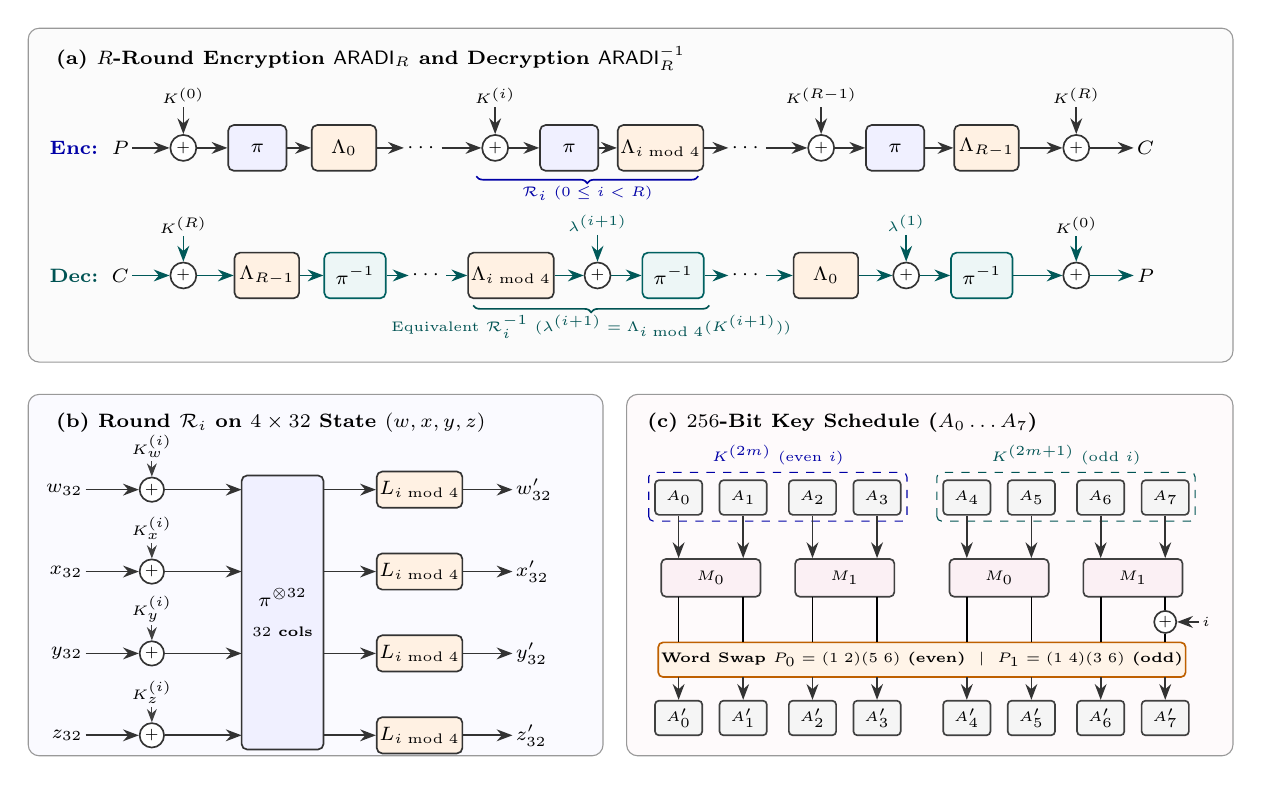
\begin{tikzpicture}[
    >=Stealth,
    sboxn/.style={rectangle, draw=black!80, semithick, rounded corners=0.7mm, fill=blue!6, minimum width=7.4mm, minimum height=5.8mm, inner sep=1pt, font=\scriptsize\bfseries},
    invsb/.style={rectangle, draw=teal!75!black, semithick, rounded corners=0.7mm, fill=teal!7, minimum width=7.8mm, minimum height=5.8mm, inner sep=1pt, font=\scriptsize\bfseries},
    linn/.style={rectangle, draw=black!80, semithick, rounded corners=0.7mm, fill=orange!11, minimum width=8.2mm, minimum height=5.8mm, inner sep=1pt, font=\scriptsize\bfseries},
    mbx/.style={rectangle, draw=black!75, semithick, rounded corners=0.6mm, fill=purple!6, minimum width=12.6mm, minimum height=4.8mm, inner sep=1pt, font=\tiny\bfseries},
    wbox/.style={rectangle, draw=black!75, semithick, rounded corners=0.5mm, fill=gray!8, minimum width=6.0mm, minimum height=4.4mm, inner sep=0.5pt, font=\tiny},
    xor/.style={circle, draw=black!80, semithick, fill=white, minimum size=3.3mm, inner sep=0pt, font=\tiny},
    lbl/.style={font=\scriptsize, inner sep=1pt},
    tlbl/.style={font=\tiny, inner sep=1pt},
    wire/.style={->, semithick, draw=black!80},
    dwire/.style={->, semithick, draw=teal!70!black}
]

% ================= PANEL (a): OVERALL ENCRYPTION & DECRYPTION SETUP =================
\begin{scope}[on background layer]
    \draw[rounded corners=1.4mm, draw=black!40, fill=gray!3] (-0.15, -1.72) rectangle (15.15, 2.52);
\end{scope}
\node[font=\scriptsize\bfseries, anchor=north west] at (0.08, 2.42) {(a) $R$-Round Encryption $\mathsf{ARADI}_R$ and Decryption $\mathsf{ARADI}_R^{-1}$};

% --- Top row: Encryption ---
\node[tlbl, font=\scriptsize\bfseries, text=blue!65!black, anchor=west] at (0.08, 1.00) {Enc:};
\node[lbl] (ep) at (1.02, 1.00) {$P$};
\node[xor] (ek0) at (1.82, 1.00) {$+$};
\node[tlbl] (ek0l) at (1.82, 1.66) {$K^{(0)}$};
\node[sboxn] (es0) at (2.76, 1.00) {$\pi$};
\node[linn]  (el0) at (3.86, 1.00) {$\Lambda_0$};
\node[lbl] (ed1) at (4.86, 1.00) {$\cdots$};

\node[xor] (eki) at (5.78, 1.00) {$+$};
\node[tlbl] (ekil) at (5.78, 1.66) {$K^{(i)}$};
\node[sboxn] (esi) at (6.72, 1.00) {$\pi$};
\node[linn]  (eli) at (7.88, 1.00) {$\Lambda_{i\bmod 4}$};
\node[lbl] (ed2) at (8.98, 1.00) {$\cdots$};

\node[xor] (ekr1) at (9.92, 1.00) {$+$};
\node[tlbl] (ekr1l) at (9.92, 1.66) {$K^{(R-1)}$};
\node[sboxn] (esr1) at (10.86, 1.00) {$\pi$};
\node[linn]  (elr1) at (12.02, 1.00) {$\Lambda_{R-1}$};
\node[xor] (ekr) at (13.16, 1.00) {$+$};
\node[tlbl] (ekrl) at (13.16, 1.66) {$K^{(R)}$};
\node[lbl] (ec) at (14.04, 1.00) {$C$};

\draw[wire] (ep) -- (ek0);
\draw[wire] (ek0l) -- (ek0);
\draw[wire] (ek0) -- (es0);
\draw[wire] (es0) -- (el0);
\draw[wire] (el0) -- (ed1);
\draw[wire] (ed1) -- (eki);
\draw[wire] (ekil) -- (eki);
\draw[wire] (eki) -- (esi);
\draw[wire] (esi) -- (eli);
\draw[wire] (eli) -- (ed2);
\draw[wire] (ed2) -- (ekr1);
\draw[wire] (ekr1l) -- (ekr1);
\draw[wire] (ekr1) -- (esr1);
\draw[wire] (esr1) -- (elr1);
\draw[wire] (elr1) -- (ekr);
\draw[wire] (ekrl) -- (ekr);
\draw[wire] (ekr) -- (ec);

\draw[decorate, decoration={brace, mirror, amplitude=2.5pt}, semithick, draw=blue!65!black]
    (5.54, 0.64) -- (8.36, 0.64) node[midway, below=2.2pt, tlbl, text=blue!65!black] {$\mathcal{R}_i$ ($0 \le i < R$)};

% --- Bottom row: Decryption & Equivalent Involution Reordering ---
\node[tlbl, font=\scriptsize\bfseries, text=teal!65!black, anchor=west] at (0.08, -0.62) {Dec:};
\node[lbl] (dc) at (1.02, -0.62) {$C$};
\node[xor] (dkr) at (1.82, -0.62) {$+$};
\node[tlbl] (dkrl) at (1.82, 0.02) {$K^{(R)}$};
\node[linn]  (dlr1) at (2.88, -0.62) {$\Lambda_{R-1}$};
\node[invsb] (dsr1) at (4.00, -0.62) {$\pi^{-1}$};
\node[lbl] (dd1) at (4.92, -0.62) {$\cdots$};

\node[linn]  (dli) at (5.98, -0.62) {$\Lambda_{i\bmod 4}$};
\node[xor]   (dki) at (7.08, -0.62) {$+$};
\node[tlbl, text=teal!70!black] (dkil) at (7.08, 0.04) {$\lambda^{(i+1)}$};
\node[invsb] (dsi) at (8.04, -0.62) {$\pi^{-1}$};
\node[lbl] (dd2) at (8.98, -0.62) {$\cdots$};

\node[linn]  (dl0) at (9.98, -0.62) {$\Lambda_0$};
\node[xor]   (dk1) at (11.00, -0.62) {$+$};
\node[tlbl, text=teal!70!black] (dk1l) at (11.00, 0.04) {$\lambda^{(1)}$};
\node[invsb] (ds0) at (11.96, -0.62) {$\pi^{-1}$};
\node[xor]   (dk0) at (13.16, -0.62) {$+$};
\node[tlbl]  (dk0l) at (13.16, 0.02) {$K^{(0)}$};
\node[lbl]   (dp) at (14.04, -0.62) {$P$};

\draw[dwire] (dc) -- (dkr);
\draw[dwire] (dkrl) -- (dkr);
\draw[dwire] (dkr) -- (dlr1);
\draw[dwire] (dlr1) -- (dsr1);
\draw[dwire] (dsr1) -- (dd1);
\draw[dwire] (dd1) -- (dli);
\draw[dwire] (dli) -- (dki);
\draw[dwire] (dkil) -- (dki);
\draw[dwire] (dki) -- (dsi);
\draw[dwire] (dsi) -- (dd2);
\draw[dwire] (dd2) -- (dl0);
\draw[dwire] (dl0) -- (dk1);
\draw[dwire] (dk1l) -- (dk1);
\draw[dwire] (dk1) -- (ds0);
\draw[dwire] (ds0) -- (dk0);
\draw[dwire] (dk0l) -- (dk0);
\draw[dwire] (dk0) -- (dp);

\draw[decorate, decoration={brace, mirror, amplitude=2.5pt}, semithick, draw=teal!65!black]
    (5.50, -1.00) -- (8.50, -1.00) node[midway, below=2.2pt, tlbl, text=teal!65!black] {Equivalent $\mathcal{R}_i^{-1}$ ($\lambda^{(i+1)} = \Lambda_{i\bmod 4}(K^{(i+1)})$)};

% ================= PANEL (b): 4 x 32 BITSLICED ROUND FUNCTION =================
\begin{scope}[yshift=-4.78cm, xshift=0.0cm]
    \draw[rounded corners=1.4mm, draw=black!40, fill=blue!2] (-0.15, -1.94) rectangle (7.15, 2.65);
    \node[font=\scriptsize\bfseries, anchor=north west] at (0.08, 2.54) {(b) Round $\mathcal{R}_i$ on $4 \times 32$ State $(w,x,y,z)$};

    \foreach \nm/\yy in {w/1.44, x/0.40, y/-0.64, z/-1.68} {
        \node[lbl, anchor=east] (in\nm) at (0.58, \yy) {$\nm_{32}$};
        \node[xor, minimum size=3.1mm] (kx\nm) at (1.42, \yy) {$+$};
        \node[tlbl, anchor=south] (kl\nm) at (1.42, \yy+0.36) {$K_\nm^{(i)}$};
        \draw[->, thin, draw=black!75] (kl\nm.south) -- (kx\nm.north);
        \node[linn, minimum width=10.2mm, minimum height=4.6mm] (ln\nm) at (4.82, \yy) {$L_{i\bmod 4}$};
        \node[lbl, anchor=west] (out\nm) at (6.00, \yy) {$\nm'_{32}$};
        \draw[wire] (in\nm) -- (kx\nm);
        \draw[wire] (kx\nm) -- (2.56, \yy);
        \draw[wire] (3.60, \yy) -- (ln\nm);
        \draw[wire] (ln\nm) -- (out\nm);
    }
    \node[sboxn, minimum width=10.4mm, minimum height=34.8mm, align=center] (sbar) at (3.08, -0.12) {$\pi^{\otimes 32}$\\[3pt]{\tiny $32$ cols}};
\end{scope}

% ================= PANEL (c): 256-BIT KEY SCHEDULE UPDATE =================
\begin{scope}[yshift=-4.78cm, xshift=7.45cm]
    \draw[rounded corners=1.4mm, draw=black!40, fill=purple!2] (0.00, -1.94) rectangle (7.70, 2.65);
    \node[font=\scriptsize\bfseries, anchor=north west] at (0.14, 2.54) {(c) $256$-Bit Key Schedule ($A_0 \dots A_7$)};

    \foreach \idx/\xx in {0/0.66, 1/1.48, 2/2.36, 3/3.18, 4/4.32, 5/5.14, 6/6.02, 7/6.84} {
        \node[wbox] (a\idx) at (\xx, 1.34) {$A_\idx$};
        \node[wbox] (b\idx) at (\xx, -1.46) {$A'_\idx$};
    }
    \draw[rounded corners=0.6mm, dashed, draw=blue!65!black] (0.28, 1.04) rectangle (3.56, 1.66);
    \node[tlbl, text=blue!65!black] at (1.92, 1.88) {$K^{(2m)}$ (even $i$)};
    \draw[rounded corners=0.6mm, dashed, draw=teal!65!black] (3.94, 1.04) rectangle (7.22, 1.66);
    \node[tlbl, text=teal!65!black] at (5.58, 1.88) {$K^{(2m+1)}$ (odd $i$)};

    \node[mbx] (m0a) at (1.07, 0.32) {$M_0$};
    \node[mbx] (m1a) at (2.77, 0.32) {$M_1$};
    \node[mbx] (m0b) at (4.73, 0.32) {$M_0$};
    \node[mbx] (m1b) at (6.43, 0.32) {$M_1$};

    \foreach \idx/\mb in {0/m0a, 1/m0a, 2/m1a, 3/m1a, 4/m0b, 5/m0b, 6/m1b, 7/m1b} {
        \draw[wire] (a\idx.south) -- (a\idx.south |- \mb.north);
    }

    \node[xor, minimum size=2.8mm] (rcx) at (6.84, -0.24) {$+$};
    \node[tlbl] (rcl) at (7.36, -0.24) {$i$};
    \draw[wire] (rcl) -- (rcx);
    \draw[semithick] (6.84, 0.08) -- (rcx);

    \node[rectangle, draw=orange!75!black, semithick, rounded corners=0.6mm, fill=orange!9, minimum width=65.4mm, minimum height=4.4mm, inner sep=1pt, font=\tiny\bfseries] (perm) at (3.75, -0.72) {Word Swap $P_0 = (1\;2)(5\;6)$ (even) $\;\mid\;$ $P_1 = (1\;4)(3\;6)$ (odd)};

    \foreach \xx in {0.66, 1.48, 2.36, 3.18, 4.32, 5.14, 6.02} {
        \draw[semithick] (\xx, 0.08) -- (\xx, -0.50);
    }
    \draw[semithick] (rcx.south) -- (6.84, -0.50);
    \foreach \idx/\xx in {0/0.66, 1/1.48, 2/2.36, 3/3.18, 4/4.32, 5/5.14, 6/6.02, 7/6.84} {
        \draw[wire] (\xx, -0.94) -- (b\idx.north);
    }
\end{scope}

\end{tikzpicture}
\caption{Specification of the $\ARADI$ block cipher~\cite{GMW24}. \textbf{(a)}~Overall $R$-round encryption $\mathsf{ARADI}_R$ (top, applying $\mathcal{R}_i(Q_i) = \Lambda_{i\bmod 4}(\pi(Q_i \oplus K^{(i)}))$ for $0 \le i < R$ and final post-whitening $K^{(R)}$) and decryption $\mathsf{ARADI}_R^{-1}$ (bottom, showing both standard decryption~\cite[Section~3.3]{GMW24} at Round~$R-1$ and the equivalent involution reordering $\mathcal{R}_i^{-1}(Q_{i+1}) = \pi^{-1}(\Lambda_{i\bmod 4}(Q_{i+1}) \oplus \lambda^{(i+1)})$ with $\lambda^{(i+1)} = \Lambda_{i\bmod 4}(K^{(i+1)})$~\cite[Figure~1]{BNS26}). \textbf{(b)}~Bitsliced round $\mathcal{R}_i$ on the four $32$-bit words $(w, x, y, z)$, applying $32$ parallel $4$-bit column S-boxes $\pi$ followed by word-wise linear involutions $L_{i\bmod 4}$. \textbf{(c)}~$256$-bit key schedule updating eight $32$-bit words $(A_0, \dots, A_7)$ via pair maps $(M_0, M_1)$, round constant $\oplus i$, and word permutation $P_{i\bmod 2}$.}
\label{fig:aradi-spec}
\end{figure}

\subsection{Law I: S-Box Quadratic Rows and Column Products}
The substitution layer $\pi$ applies the same $4$-bit S-box independently to all $32$ columns via four sequential word-wise Toffoli gates~\cite[Figure~3.1, p.~4]{GMW24}.
\begin{equation}
\label{eq:sbox-seq}
x \leftarrow x \oplus (w \wedge y), \qquad
z \leftarrow z \oplus (x \wedge y), \qquad
y \leftarrow y \oplus (w \wedge z), \qquad
w \leftarrow w \oplus (x \wedge z).
\end{equation}
Evaluating~\eqref{eq:sbox-seq} on $v = 8w + 4x + 2y + z \in \{0,\dots,15\}$ yields the hexadecimal lookup tables
\[
\begin{aligned}
\pi[0 \dots 15] &= [\texttt{0, 1, 2, 3, 4, D, F, 6, 8, B, 5, E, C, 7, A, 9}], \\
\pi^{-1}[0 \dots 15] &= [\texttt{0, 1, 2, 3, 4, A, 7, D, 8, F, E, 9, C, 5, B, 6}].
\end{aligned}
\]
Expanding~\eqref{eq:sbox-seq} over $\Ftwo[w,x,y,z]/(w^2{-}w, x^2{-}x, y^2{-}y, z^2{-}z)$ using $y^2 = y$ in step~2 gives the S-box ANF~\cite{BFG24,BRRT25,DG25} underlying Structural Law~I exploited by $\OPTIC$.
\begin{equation}
\label{eq:sbox-anf}
\begin{aligned}
\pi_w &= w \oplus wy \oplus xy \oplus xz \oplus wyz \;\;(\deg = 3), &
\pi_x &= x \oplus wy \;\;(\mathbf{\deg = 2}), \\
\pi_y &= y \oplus wy \oplus wz \oplus wxy \;\;(\deg = 3), &
\pi_z &= z \oplus xy \oplus wy \;\;(\mathbf{\deg = 2}).
\end{aligned}
\end{equation}
Three algebraic properties of~\eqref{eq:sbox-anf} drive Module~I:
\begin{enumerate}[label=(I.\arabic*),leftmargin=2.2em,nosep]
    \item \textbf{Quadratic Row Pullback ($\deg \pi_x = \deg \pi_z = 2$~\cite{BRRT25}):} Whereas $\pi_w$ and $\pi_y$ have degree~$3$, rows $x$ and $z$ are purely quadratic, and their sum $\pi_x \oplus \pi_z = x \oplus z \oplus xy$ eliminates $wy$ to leave a single quadratic monomial $xy$~\cite{BRRT25}.
    \item \textbf{First-Round Single-Bit and $(y,z)$-Pair Affinity:} Activating any single bit (such as $y_b$) in column~$b$ traverses Round~$0$'s S-box with degree~$\le 1$. Also, because $yz$ is absent from $\pi_x, \pi_y, \pi_z$ in~\eqref{eq:sbox-anf}, activating $(y_b, z_b)$ simultaneously still keeps $\pi_x, \pi_y, \pi_z$ purely affine ($\deg \le 1$) and introduces only $w_b y_b z_b$ in $\pi_w$.
    \item \textbf{Degree-$3$ Intra-Column Product Cancellation ($\deg(\pi_r \pi_s) \le 3$~\cite{BC11}):} By the classical degree bound on coordinate products of bijections on $\Ftwo^4$~\cite{BC11}, every product of two distinct coordinates within the \emph{same} column $b$ has even truth-table weight~$4$. That cancels $wxyz$ identically: $\pi_w \pi_y = xy \oplus wz \oplus wxz \oplus xyz$ and $(\pi_x \oplus \pi_w)\pi_y = wz \oplus wxy \oplus wyz \oplus xyz$ ($\deg = 3$). By contrast, a cross-column product $\pi_w(U_b)\pi_y(U_{b'})$ ($b \neq b'$) has degree $3 + 3 = 6$.
\end{enumerate}

\subsection{Law II: Linear Involutions and \texorpdfstring{$L_3$}{L\_3} Orthogonality}
In round $i$, the layer $\Lambda_{i \bmod 4}(w,x,y,z)$ applies $L_j$ ($j = i \bmod 4$) word-wise to each $32$-bit word $W = u \parallel l$ ($u, l \in \Ftwo^{16}$)~\cite[Figure~3.2, p.~5]{GMW24}:
\begin{equation}
\label{eq:Lj}
L_j(u \parallel l) = \Bigl(u \oplus \ROL_{16}(u, a_j) \oplus \ROL_{16}(l, c_j)\Bigr) \;\Big\|\; \Bigl(l \oplus \ROL_{16}(l, a_j) \oplus \ROL_{16}(u, b_j)\Bigr),
\end{equation}
with published rotation triples $(a_0,b_0,c_0) = (11,8,14)$, $(a_1,b_1,c_1) = (10,9,11)$, $(a_2,b_2,c_2) = (9,4,14)$, and $(a_3,b_3,c_3) = (8,9,7)$. Writing $R = \ROL_{16}(\cdot, 1)$ ($R^{16} = I_{16}$), $L_j$ has block-circulant matrix form
\begin{equation}
\label{eq:Lj-block}
L_j = \begin{pmatrix} I_{16} + R^{a_j} & R^{c_j} \\ R^{b_j} & I_{16} + R^{a_j} \end{pmatrix}, \qquad
L_j^\top = \begin{pmatrix} I_{16} + R^{-a_j} & R^{-b_j} \\ R^{-c_j} & I_{16} + R^{-a_j} \end{pmatrix}.
\end{equation}
Equation~\eqref{eq:Lj-block} yields the three properties constituting Structural Law~II:
\begin{enumerate}[label=(II.\arabic*),leftmargin=2.2em,nosep]
    \item \textbf{Row-Weight-$3$ Involution Decoupling ($L_j^2 = I_{32}$~\cite{GMW24}):} As designed in~\cite[Section~3.1, p.~5]{GMW24}, because $2a_j \equiv b_j + c_j \pmod{16}$ holds for all four triples ($6\equiv 6, 4\equiv 4, 2\equiv 2, 0\equiv 0$), $L_j^2 = \operatorname{diag}(I_{16}+R^{2a_j}+R^{b_j+c_j}, I_{16}+R^{2a_j}+R^{b_j+c_j}) = I_{32}$. Following standard equivalent-subkey peeling~\cite{BRRT25,BBGHP25,DG25}, left-multiplying ciphertext $C = \Lambda_{R-1}(\pi(Q_{R-1}\oplus K^{(R-1)})) \oplus K^{(R)}$ by $\Lambda_{R-1}$ gives
    \begin{equation}
    \label{eq:peel}
    T(P) := \Lambda_{R-1}\bigl(C(P)\bigr) = \pi\bigl(Q_{R-1}(P) \oplus K^{(R-1)}\bigr) \oplus \lambda, \qquad \lambda := \Lambda_{R-1}(K^{(R)}),
    \end{equation}
    decoupling the outer S-box layer into $32$ independent $4$-bit columns $Y_{\uparrow b}(P) = \pi^{-1}(T_{\uparrow b}(P) \oplus \lambda_{\uparrow b})$.
    \item \textbf{Unique Orthogonality and $8$-Island Split of $L_3 = (8,9,7)$:} By~\eqref{eq:Lj-block}, $L_j^\top L_j = I_{32} \iff L_j^\top = L_j \iff 2a_j \equiv b_j + c_j \equiv 0 \pmod{16}$, which holds \emph{uniquely} for $j = 3$. In addition, strengthening the rotation-$8$ byte-wise cancellation noted in~\cite{BFG24,KKL24}, $\gcd(a_3, 16) = \gcd(8, 16) = 8$ and $b_3 \equiv -c_3 \equiv 1 \pmod 8$ partition $\{0,\dots,31\}$ into eight disjoint $L_3$-invariant $4$-column islands:
    \begin{equation}
    \label{eq:islands}
    G_g = \bigl\{g,\; g+8,\; 16 + ((g+7)\bmod 16),\; 16 + ((g+15)\bmod 16)\bigr\} \qquad (0 \le g \le 7).
    \end{equation}
    \item \textbf{Half-Word Transpose Asymmetry of $L_0, L_1, L_2$ ($b_j \not\equiv -c_j \pmod{16}$):} Swapping the upper half $u$ and lower half $l$ conjugates $L_j$ by $\bigl(\begin{smallmatrix}0 & I\\ I & 0\end{smallmatrix}\bigr)$, exchanging $b_j \leftrightarrow c_j$. Because $b_j \neq c_j$ for all $j$ and $b_j + c_j \not\equiv 0 \pmod{16}$ for $j \in \{0,1,2\}$, multi-round cones are \emph{asymmetric between $\{16,\dots,31\}$ and $\{0,\dots,15\}$}. A $3$-round forward cone from column~$c_0$ covers $23$ columns if $c_0 < 16$ vs.\ $22$ if $c_0 \ge 16$. Denoting by $T_r(c) \subseteq \{0,\dots,31\}$ the set of active subkey columns at round~$r$ in the backward dependency cone of column~$c$, a $4$-round backward cone at Round~$12$ has leaf width $|T_{12}(c)| = 22$ for all $c \in \{0,\dots,15\}$ vs.\ $|T_{12}(c)| = 23$ for all $c \in \{16,\dots,31\}$. This also explains the $2$--$3$-round key-cone asymmetry in~\cite[$\S$5.1, Table~5]{BNS26} (Section~\ref{subsec:tosc-comparison}).
\end{enumerate}

\begin{figure}[t!]
\centering
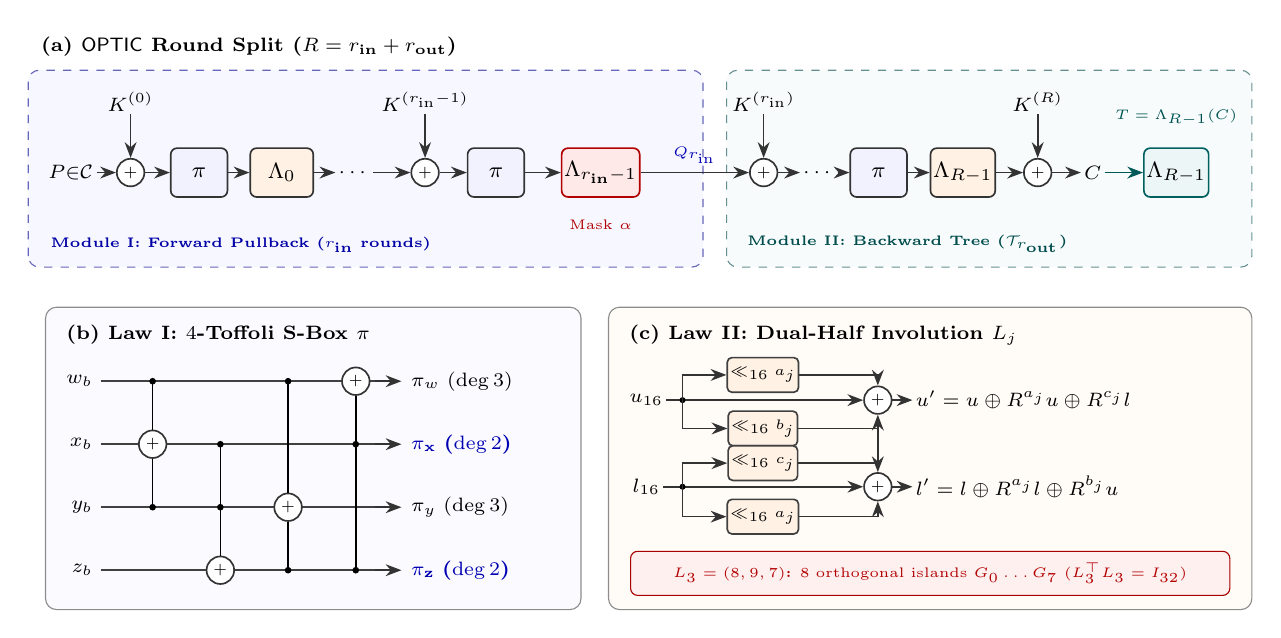
\begin{tikzpicture}[
    >=Stealth,
    sboxn/.style={rectangle, draw=black!80, semithick, rounded corners=0.8mm, fill=blue!5, minimum width=7.2mm, minimum height=6.2mm, inner sep=1pt, font=\footnotesize\bfseries},
    linn/.style={rectangle, draw=black!80, semithick, rounded corners=0.8mm, fill=orange!11, minimum width=8.0mm, minimum height=6.2mm, inner sep=1pt, font=\footnotesize\bfseries},
    invn/.style={rectangle, draw=teal!75!black, semithick, rounded corners=0.8mm, fill=teal!7, minimum width=8.2mm, minimum height=6.2mm, inner sep=1pt, font=\footnotesize\bfseries},
    rotb/.style={rectangle, draw=black!75, semithick, rounded corners=0.6mm, fill=orange!10, minimum width=8.6mm, minimum height=4.4mm, inner sep=1pt, font=\tiny},
    xor/.style={circle, draw=black!80, semithick, fill=white, minimum size=3.5mm, inner sep=0pt, font=\tiny},
    lbl/.style={font=\scriptsize, inner sep=1pt},
    tlbl/.style={font=\tiny, inner sep=1pt},
    wire/.style={->, semithick, draw=black!80},
    peelwire/.style={->, semithick, draw=teal!70!black}
]

% ================= PANEL (a): R-ROUND ARADI + OPTIC PIPELINE =================
\node[font=\scriptsize\bfseries, anchor=west] at (-0.18, 2.18) {(a) $\OPTIC$ Round Split ($R = r_{\text{in}} + r_{\text{out}}$)};

\begin{scope}[on background layer]
    \draw[rounded corners=1.4mm, dashed, draw=blue!55!black!60, fill=blue!3] (-0.22, -0.62) rectangle (8.35, 1.88);
    \node[font=\tiny\bfseries, text=blue!65!black, anchor=south west] at (-0.06, -0.56) {Module I: Forward Pullback ($r_{\text{in}}$ rounds)};
    \draw[rounded corners=1.4mm, dashed, draw=teal!55!black!60, fill=teal!3] (8.65, -0.62) rectangle (15.32, 1.88);
    \node[font=\tiny\bfseries, text=teal!60!black, anchor=south west] at (8.79, -0.56) {Module II: Backward Tree ($\mathcal{T}_{r_{\text{out}}}$)};
\end{scope}

\node[lbl] (p0) at (0.32, 0.58) {$P{\in}\mathcal{C}$};
\node[xor] (kx0) at (1.08, 0.58) {$+$};
\node[lbl] (k0) at (1.08, 1.48) {$K^{(0)}$};
\node[sboxn] (s0) at (1.95, 0.58) {$\pi$};
\node[linn]  (l0) at (3.00, 0.58) {$\Lambda_0$};

\node[lbl] (dots) at (3.92, 0.58) {$\cdots$};

\node[xor] (kx4) at (4.82, 0.58) {$+$};
\node[lbl] (k4) at (4.82, 1.48) {$K^{(r_{\text{in}}-1)}$};
\node[sboxn] (s4) at (5.72, 0.58) {$\pi$};
\node[linn, fill=red!9, draw=red!70!black] (l3) at (7.05, 0.58) {$\Lambda_{r_{\text{in}}-1}$};
\node[tlbl, text=red!70!black] at (7.05, -0.08) {Mask $\alpha$};

\node[xor] (kx5) at (9.12, 0.58) {$+$};
\node[lbl] (k5) at (9.12, 1.48) {$K^{(r_{\text{in}})}$};
\node[lbl] (dots2) at (9.82, 0.58) {$\cdots$};

\node[sboxn] (s5) at (10.58, 0.58) {$\pi$};
\node[linn]  (l5) at (11.65, 0.58) {$\Lambda_{R-1}$};
\node[xor]   (kx6) at (12.60, 0.58) {$+$};
\node[lbl]   (k6) at (12.60, 1.48) {$K^{(R)}$};
\node[lbl]   (c0) at (13.30, 0.58) {$C$};
\node[invn]  (linv) at (14.36, 0.58) {$\Lambda_{R-1}$};
\node[tlbl, text=teal!65!black] at (14.36, 1.28) {$T = \Lambda_{R-1}(C)$};

\draw[wire] (p0) -- (kx0);
\draw[wire] (k0) -- (kx0);
\draw[wire] (kx0) -- (s0);
\draw[wire] (s0) -- (l0);
\draw[wire] (l0) -- (dots);
\draw[wire] (dots) -- (kx4);
\draw[wire] (k4) -- (kx4);
\draw[wire] (kx4) -- (s4);
\draw[wire] (s4) -- (l3);
\draw[wire] (l3) -- node[tlbl, above=2pt, text=blue!70!black] {$Q_{r_{\text{in}}}$} (kx5);
\draw[wire] (k5) -- (kx5);
\draw[wire] (kx5) -- (dots2);
\draw[wire] (dots2) -- (s5);
\draw[wire] (s5) -- (l5);
\draw[wire] (l5) -- (kx6);
\draw[wire] (k6) -- (kx6);
\draw[wire] (kx6) -- (c0);
\draw[peelwire] (c0) -- (linv);

% ================= PANEL (b): 4-TOFFOLI S-BOX CIRCUIT (LAW I) =================
\begin{scope}[yshift=-3.45cm, xshift=0.0cm]
    \draw[rounded corners=1.4mm, draw=black!45, fill=blue!2] (0.00, -1.52) rectangle (6.80, 2.32);
    \node[font=\scriptsize\bfseries, anchor=north west] at (0.14, 2.22) {(b) Law I: $4$-Toffoli S-Box $\pi$};

    \foreach \nm/\yy in {w/1.38, x/0.58, y/-0.22, z/-1.02} {
        \node[lbl, anchor=east] at (0.64, \yy) {$\nm_b$};
        \draw[semithick, draw=black!75] (0.70, \yy) -- (4.22, \yy);
    }
    \node[xor] (g1) at (1.36, 0.58) {$+$};
    \fill (1.36, 1.38) circle (1.2pt);
    \fill (1.36, -0.22) circle (1.2pt);
    \draw[semithick] (1.36, 1.38) -- (g1);
    \draw[semithick] (1.36, -0.22) -- (g1);

    \node[xor] (g2) at (2.22, -1.02) {$+$};
    \fill (2.22, 0.58) circle (1.2pt);
    \fill (2.22, -0.22) circle (1.2pt);
    \draw[semithick] (2.22, 0.58) -- (g2);
    \draw[semithick] (2.22, -0.22) -- (g2);

    \node[xor] (g3) at (3.08, -0.22) {$+$};
    \fill (3.08, 1.38) circle (1.2pt);
    \fill (3.08, -1.02) circle (1.2pt);
    \draw[semithick] (3.08, 1.38) -- (g3);
    \draw[semithick] (3.08, -1.02) -- (g3);

    \node[xor] (g4) at (3.94, 1.38) {$+$};
    \fill (3.94, 0.58) circle (1.2pt);
    \fill (3.94, -1.02) circle (1.2pt);
    \draw[semithick] (3.94, 0.58) -- (g4);
    \draw[semithick] (3.94, -1.02) -- (g4);

    \draw[wire] (4.18, 1.38) -- (4.52, 1.38);
    \draw[wire] (4.18, 0.58) -- (4.52, 0.58);
    \draw[wire] (4.18, -0.22) -- (4.52, -0.22);
    \draw[wire] (4.18, -1.02) -- (4.52, -1.02);

    \node[lbl, anchor=west] at (4.60, 1.38) {$\pi_w$ ($\deg 3$)};
    \node[lbl, anchor=west, text=blue!70!black] at (4.60, 0.58) {$\mathbf{\pi_x}$ \textbf{($\deg 2$)}};
    \node[lbl, anchor=west] at (4.60, -0.22) {$\pi_y$ ($\deg 3$)};
    \node[lbl, anchor=west, text=blue!70!black] at (4.60, -1.02) {$\mathbf{\pi_z}$ \textbf{($\deg 2$)}};
\end{scope}

% ================= PANEL (c): DUAL-HALF INVOLUTION L_j & L_3 ISLANDS (LAW II) =================
\begin{scope}[yshift=-3.45cm, xshift=7.15cm]
    \draw[rounded corners=1.4mm, draw=black!45, fill=orange!3] (0.00, -1.52) rectangle (8.17, 2.32);
    \node[font=\scriptsize\bfseries, anchor=north west] at (0.14, 2.22) {(c) Law II: Dual-Half Involution $L_j$};

    \node[lbl] (uin) at (0.48, 1.14) {$u_{16}$};
    \node[lbl] (lin) at (0.48, 0.04) {$l_{16}$};
    \node[rotb] (ra1) at (1.96, 1.46) {$\ll_{16} a_j$};
    \node[rotb] (rb)  at (1.96, 0.78) {$\ll_{16} b_j$};
    \node[rotb] (rc)  at (1.96, 0.34) {$\ll_{16} c_j$};
    \node[rotb] (ra2) at (1.96, -0.34) {$\ll_{16} a_j$};

    \node[xor] (xu) at (3.42, 1.14) {$+$};
    \node[xor] (xl) at (3.42, 0.04) {$+$};
    \node[lbl, anchor=west] (uout) at (3.86, 1.14) {$u' = u \oplus R^{a_j}u \oplus R^{c_j}l$};
    \node[lbl, anchor=west] (lout) at (3.86, 0.04) {$l' = l \oplus R^{a_j}l \oplus R^{b_j}u$};

    \draw[wire] (uin) -- (xu);
    \draw[wire] (lin) -- (xl);
    \fill (0.94, 1.14) circle (1.1pt);
    \fill (0.94, 0.04) circle (1.1pt);
    \draw[wire] (0.94, 1.14) |- (ra1.west);
    \draw[wire] (0.94, 1.14) |- (rb.west);
    \draw[wire] (0.94, 0.04) |- (rc.west);
    \draw[wire] (0.94, 0.04) |- (ra2.west);
    \draw[wire] (ra1.east) -| (xu.north);
    \draw[wire] (rc.east)  -| (xu.south);
    \draw[wire] (rb.east)  -| (xl.north);
    \draw[wire] (ra2.east) -| (xl.south);
    \draw[wire] (xu) -- (uout);
    \draw[wire] (xl) -- (lout);

    \draw[rounded corners=0.9mm, draw=red!65!black, fill=red!6] (0.28, -1.34) rectangle (7.89, -0.78);
    \node[tlbl, text=red!70!black] at (4.085, -1.06) {\textbf{$L_3=(8,9,7)$:} $8$ orthogonal islands $G_0\dots G_7$ ($L_3^\top L_3 = I_{32}$)};
\end{scope}

\end{tikzpicture}
\caption{Structure of $\ARADI$~\cite{GMW24} and the $\OPTIC$ round split. \textbf{(a)}~Partitioning $R = r_{\text{in}} + r_{\text{out}}$ rounds into Module~I (pulling mask $\alpha = \Lambda_{r_{\text{in}}-1}^\top(\beta \otimes \nu)$ onto quadratic S-box rows at $Q_{r_{\text{in}}}$) and Module~II (peeling the depth-$r_{\text{out}}$ ternary tree $\mathcal{T}_{r_{\text{out}}}$ from $T = \Lambda_{R-1}(C)$). \textbf{(b)}~Sequential $4$-Toffoli-gate S-box $\pi$~\eqref{eq:sbox-anf}, whose second and fourth outputs $\pi_x, \pi_z$ have degree~$2$. \textbf{(c)}~Dual-half involution $L_j$~\eqref{eq:Lj}; for $j=3$, $L_3$ splits into eight orthogonal $4$-column islands~\eqref{eq:islands}.}
\label{fig:aradi-arch}
\end{figure}

\subsection{Law III: Even-Pair Key-Schedule Inversion}
The $256$-bit master key initializes eight $32$-bit register words $(A_0, \dots, A_7)$. In round $i \in \{0, \dots, 15\}$, let $j = i \bmod 2$; the round key is extracted \emph{prior} to updating the register as
\[
K^{(i)} = (A_0, A_1, A_2, A_3) \text{ if } i \text{ is even}, \qquad
K^{(i)} = (A_4, A_5, A_6, A_7) \text{ if } i \text{ is odd},
\]
with post-whitening key $K^{(R)}$ extracted from half $j = R \bmod 2$ after $R$ register updates. Each update applies the invertible $\Ftwo$-linear pair maps $M_0(X,Y) = \bigl(\ROL_{32}(X,1)\oplus Y,\; \ROL_{32}(Y,3)\oplus\ROL_{32}(X,1)\oplus Y\bigr)$ to $(A_0,A_1)$ and $(A_4,A_5)$, and $M_1(X,Y) = \bigl(\ROL_{32}(X,9)\oplus Y,\; \ROL_{32}(Y,28)\oplus\ROL_{32}(X,9)\oplus Y\bigr)$ to $(A_2,A_3)$ and $(A_6,A_7)$, XORs the round counter $i$ into $A_7$, and applies the word swap $P_0 = (1\;2)(5\;6)$ (even $i$) or $P_1 = (1\;4)(3\;6)$ (odd $i$)~\cite[Section~3.2, p.~7; Figure~3.3, p.~6; Figure~3.5, p.~8]{GMW24}. Algorithm~1 summarizes the complete $R$-round encryption and key schedule.

\begin{figure}[t]
\centering
\small
\begin{tabular}{@{}p{0.97\textwidth}@{}}
\toprule
\textbf{Algorithm 1:} $R$-Round $\ARADI$ Key Schedule, Encryption, and Even-Pair Master-Key Inversion~\cite{GMW24,DG25} \\
\midrule
\textbf{Key Expansion $\mathsf{ARADI\text{-}KS}(A_0 \dots A_7, R)$:} \\
\hspace*{1.2em} \textbf{1.} \textbf{for} $i = 0$ \textbf{to} $R - 1$ \textbf{do} \quad $j \leftarrow i \bmod 2$; \quad $K^{(i)} \leftarrow (A_{4j}, A_{4j+1}, A_{4j+2}, A_{4j+3})$; \\
\hspace*{2.8em} $(A_0, A_1) \leftarrow M_0(A_0, A_1)$; $\;(A_2, A_3) \leftarrow M_1(A_2, A_3)$; $\;(A_4, A_5) \leftarrow M_0(A_4, A_5)$; $\;(A_6, A_7) \leftarrow M_1(A_6, A_7)$; \\
\hspace*{2.8em} $A_7 \leftarrow A_7 \oplus i$; \quad \textbf{if} $j = 0$ \textbf{then} $\mathsf{swap}(A_1,A_2),\, \mathsf{swap}(A_5,A_6)$ \textbf{else} $\mathsf{swap}(A_1,A_4),\, \mathsf{swap}(A_3,A_6)$; \\
\hspace*{1.2em} \textbf{2.} $j \leftarrow R \bmod 2$; \quad $K^{(R)} \leftarrow (A_{4j}, A_{4j+1}, A_{4j+2}, A_{4j+3})$; \quad \textbf{return} $(K^{(0)}, \dots, K^{(R)})$. \\[3pt]
\midrule
\textbf{Encryption $\mathsf{ARADI}_R(P, K^{(0 \dots R)})$:} \hfill (retaining all $R$ linear layers and post-whitening $K^{(R)}$) \\
\hspace*{1.2em} \textbf{1.} $Q_0 \leftarrow P$; \quad \textbf{for} $i = 0$ \textbf{to} $R - 1$ \textbf{do} $Q_{i+1} \leftarrow \Lambda_{i \bmod 4}\bigl(\pi(Q_i \oplus K^{(i)})\bigr)$; \quad \textbf{return} $C \leftarrow Q_R \oplus K^{(R)}$. \\[3pt]
\midrule
\textbf{Closed-Form Master-Key Inversion $\mathsf{KS}^{-1}(K^{(2m)}, K^{(2m+1)}, 2m)$~\cite[Remark~5]{DG25}:} \hfill ($O(1)$ ops for even $2m$) \\
\hspace*{1.2em} \textbf{1.} Parse $K^{(2m+1)} = (U_4, U_6, U_5, U_7')$; \quad $U_7 \leftarrow U_7' \oplus 2m$; \hfill $\triangleright\;$ undo $P_0 = (1\;2)(5\;6)$ and counter XOR \\
\hspace*{1.2em} \textbf{2.} $(A_4, A_5) \leftarrow M_0^{-1}(U_4, U_5)$; \quad $(A_6, A_7) \leftarrow M_1^{-1}(U_6, U_7)$; \quad $S^{(2m)} \leftarrow K^{(2m)} \,\|\, (A_4, A_5, A_6, A_7)$; \\
\hspace*{1.2em} \textbf{3.} \textbf{for} $i = 2m - 1$ \textbf{downto} $0$ \textbf{do} invert step~$i$ on $S^{(i+1)}$ via $P_{i\bmod 2}^{-1}$, $A_7 \oplus i$, and $(M_0^{-1}, M_1^{-1})$; \textbf{return} $S^{(0)}$. \\
\bottomrule
\end{tabular}
\end{figure}

Structural Law~III powers Module~III of $\OPTIC$, formalizing the even-pair invertibility noted by Dunkelman and Ghosh~\cite[Remark~5]{DG25} and the $\Ftwo$-affine subkey rank relations used in~\cite{DG25,GMNP25,BNS26,LST26}:
\begin{enumerate}[label=(III.\arabic*),leftmargin=2.2em,nosep]
    \item \textbf{Even-Pair $O(1)$ Direct-Sum Closure:} At an \emph{even} round $2m$, $P_0 = (1\;2)(5\;6)$ preserves the partition between the lower half $(A_0,\dots,A_3)$ and upper half $(A_4,\dots,A_7)$. Hence any even-indexed consecutive subkey pair $(K^{(2m)}, K^{(2m+1)})$---such as $(K^{(2)}, K^{(3)})$ at $5$R, $(K^{(4)}, K^{(5)})$ at $6$R, $(K^{(6)}, K^{(7)})$ at $7$--$8$R, $(K^{(8)}, K^{(9)})$ at $9$--$11$R, or $(K^{(10)}, K^{(11)})$ at $12$R---uniquely reconstructs the $256$-bit master key via $\mathsf{KS}^{-1}$ in $O(1)$ word operations with zero brute-force search. Conversely, an odd-indexed pair $(K^{(2m-1)}, K^{(2m)})$ spans only $192$ master-key bits because $P_1 = (1\;4)(3\;6)$ swaps two $32$-bit words between the register halves.
    \item \textbf{Cross-Round Affine Consistency ($128k - 256$ Equations):} Because every $K^{(i)}$ is an $\Ftwo$-affine image of the $256$-bit master key, any $k \ge 3$ consecutive round keys satisfy $128k - 256$ exact $\Ftwo$-affine consistency equations ($256$ equations across $K^{(2)}, K^{(3)}, K^{(4)}, K^{(5)}$).
\end{enumerate}

\section{Module I: Forward Pullback Distinguishers}
\label{sec:forward-engine}
\label{sec:5round}
\label{sec:6round}

The first half of the $\OPTIC$ pipeline constructs universal, key-independent zero-sum identities at internal state $Q_{r_{\text{in}}}$ using minimum plaintext data $D = |\mathcal{C}|$. Rather than designing separate truncated-differential, super-S-box, null-space, and Toffoli distinguishers, Module~I unifies all four under a single mechanism. Given a $d$-dimensional cube (or prefix) $\mathcal{C} \subset \Ftwo^{128}$ and a pulled-back linear mask
\begin{equation}
\label{eq:unified-pullback}
\alpha = \Lambda_{r_{\text{in}}-1}^\top(\beta \otimes \nu) \in \Ftwo^{128} \qquad \bigl(\beta \in \Ftwo^{32},\;\; \nu \in \spanF\{e_x, e_z\}\bigr),
\end{equation}
Law~II.1 ($\Lambda_{r_{\text{in}}-1}^2 = I_{128}$) pulls the inner product across $\Lambda_{r_{\text{in}}-1}$ directly onto the quadratic S-box rows $\pi_x, \pi_z$ of Round~$r_{\text{in}}-1$.
\[
\bigoplus_{P \in \mathcal{C}} \bigl\langle \alpha,\; Q_{r_{\text{in}}}(P) \bigr\rangle
= \bigoplus_{P \in \mathcal{C}} \bigoplus_{b \in \supp(\beta)} \bigl\langle \nu,\; \pi\bigl(Q_{r_{\text{in}}-1,\uparrow b}(P) \oplus K^{(r_{\text{in}}-1)}_{\uparrow b}\bigr) \bigr\rangle.
\]
As $r_{\text{in}}$ increases from $1$ to $8$, this pullback operates across four progressive degree-compression regimes (Regimes~I--IV).

\subsection{Regime I: Difference Subspaces and Blind-Column Audit}
\label{subsec:regime1}

When $d = 1$, $\mathcal{C} = \{P, P \oplus \Delta P\}$ is a single plaintext pair, and $\bigoplus_{P \in \mathcal{C}} \langle \alpha, Q_k(P)\rangle = \langle \alpha, \Delta Q_k\rangle$. If $\Delta P$ is supported on a single column $c_0$, then $\Delta Q_k$ is confined to a deterministic subspace $V_k(c_0) \subset \Ftwo^{128}$ of dimension
\[
\dim V_1 = 3,\qquad \dim V_2 = 12,\qquad \dim V_3 = 36,\qquad \dim V_4 = 88 \text{ or } 92,
\]
so every mask $\alpha \in V_k(c_0)^\perp$ (codimensions $125, 116, 92, 40/36$) satisfies $\bigoplus_{P \in \mathcal{C}} \langle \alpha, Q_k(P)\rangle = 0$ unconditionally for all keys. However, if one restricts $\alpha$ at $r_{\text{in}} = 3$ only to dead-column masks $e_k \otimes \nu$ ($k \in \mathcal{D}_3(c_0)$ where $\Delta Q_{3,\uparrow k} = 0$) as in Bellini et al.~\cite[$\S$6.2]{BBGHP25}, Law~II.2--II.3 imposes a strict information-theoretic blind-column defect:

\begin{proposition}[Blind-Column Defect in Single-Difference $5$-Round Truncated Differentials]
\label{prop:blind-cols}
Let $R = 5$ ($r_0 = 0$). For every single-column input difference $\Delta P$ active solely in column $c_0 \in \{0, \dots, 31\}$, deterministic propagation through $\Lambda_0, \Lambda_1, \Lambda_2$ leaves $|\mathcal{D}_3(c_0)| = 9$ inactive (``dead'') columns entering Round~$3$ if $0 \le c_0 \le 15$ and $|\mathcal{D}_3(c_0)| = 10$ if $16 \le c_0 \le 31$. Because $\Lambda_3$ ($L_3$ with $(a_3,b_3,c_3)=(8,9,7)$, $\gcd(8,16)=8$) partitions $\{0,\dots,31\}$ into the eight disjoint $4$-column islands $G_0, \dots, G_7$ in~\eqref{eq:islands}, the backward dependency union $\bigcup_{k \in \mathcal{D}_3(c_0)} \supp_k(L_3)$ covers exactly $19$ columns of $\lambda = \Lambda_0(K^{(5)})$ for $0 \le c_0 \le 15$ and $24$ columns for $16 \le c_0 \le 31$, leaving $13$ or $8$ ``blind'' columns ($52$ or $32$ bits of $K^{(5)}$) completely unconstrained regardless of how many plaintext pairs are queried along $\Delta P$.
\end{proposition}

\begin{proof}
\emph{Proof idea:} We first trace the $3$-round forward diffusion cone of column~$c_0$ to identify all inactive columns entering Round~$3$, and then intersect those inactive columns with the eight $L_3$-invariant $4$-column islands $G_0, \dots, G_7$. Any island containing zero inactive columns imposes no dead-column constraints on its four subkey nibbles in $\lambda$.

Direct evaluation of $\supp(L_2(L_1(L_0(e_{c_0}))))$ for each $c_0 \in \{0,\dots,31\}$ yields $23$ active columns ($9$ dead) when $c_0 < 16$ and $22$ active columns ($10$ dead) when $c_0 \ge 16$ (by the half-word asymmetry of Law~II.3). Under $L_3$, any shift by $a_3 = 8 \bmod 16$ preserves residue modulo~$8$ in both $16$-bit halves. Meanwhile, $b_3 = 9 \equiv 1 \pmod 8$ and $c_3 = 7 \equiv -1 \pmod 8$ pair lower-half pair $\{g, g+8\}$ exclusively with upper-half pair $\{16+((g+7)\bmod 16), 16+((g+15)\bmod 16)\}$, partitioning $\{0,\dots,31\}$ into the eight $L_3$-invariant $4$-column islands $G_0, \dots, G_7$. For every $c_0 \ge 16$, two of the eight islands contain zero dead columns in $\mathcal{D}_3(c_0)$, leaving $2 \times 4 = 8$ columns of $\lambda$ outside $\bigcup_{k \in \mathcal{D}_3(c_0)}\supp_k(L_3)$ ($13$ columns when $c_0 < 16$). Thus the $10$-pair ($20\text{-}\CP$) single-difference procedure of~\cite[Section~6.2]{BBGHP25} requires at least two distinct input differences ($40~\CP$) to cover all $32$ columns. By contrast, choosing $3$ pairs along complementary single-bit directions covers all $8$ islands with zero blind columns at $6~\CP$.
\end{proof}

\subsection{Regime II: Two-Round Orthogonal-Island Collapse}
\label{subsec:regime2}

At $r_{\text{in}} = 5$ inner rounds ($Q_0 \to Q_5$, required for $6$-round peeling), Regime~I subspaces saturate completely ($\dim V_5 = 128$, zero dead columns). Every individual coordinate of $Q_5$ or $Z_4 = \Lambda_0(Q_5) = \pi(Q_4 \oplus K^{(4)})$ reaches full algebraic degree~$6$ on a $6$D cube. This matches Kim et al.'s $2^{77}\text{-}\CP$ $6$-round division-property bound~\cite{KKL24} and Beyne et al.'s $2^{-82}$ $6$-round differential bound~\cite[Appendix~A]{BNS26}.

Module~I breaks this degree-$6$ barrier by setting the pullback mask in~\eqref{eq:unified-pullback} to the $4$-column island indicator $\beta = \mathbf{1}_{G_g}$ and $\nu \in \{e_x, e_z\}$. Combining Law~I.1, Law~I.3, and Law~II.2 ($L_3^\top L_3 = I_{32}$) collapses \emph{two consecutive rounds} $S_3 \to \Lambda_3 \to S_4$ into a single degree-$3$ super-S-box.

\begin{theorem}[Orthogonal-Island Super-S-Box Collapse across $S_3 \to \Lambda_3 \to S_4$]
\label{thm:orth-collapse}
Among the four linear maps $L_0, L_1, L_2, L_3$ of $\ARADI$~\eqref{eq:Lj}, $L_3$ with $(a_3, b_3, c_3) = (8, 9, 7)$ is the \emph{unique} symmetric and orthogonal binary matrix ($L_3^\top = L_3$ and $L_3^\top L_3 = I_{32}$), whereas $L_0, L_1, L_2$ admit zero non-trivial cross-column product-canceling masks in $\Ftwo^{32}$. Specifically:
\begin{enumerate}[leftmargin=1.8em]
    \item \textbf{Island-Wise Bilinear Inner-Product Invariance:} On each of the eight disjoint $4$-column islands $G_g \subset \{0,\dots,31\}$ ($0 \le g \le 7$) in~\eqref{eq:islands}, for any Boolean polynomial vectors $A, B \in \bigl(\Ftwo[u_0,\dots,u_{d-1}]\bigr)^{32}$,
    \begin{equation}
    \label{eq:orth-cancel}
    \bigoplus_{b \in G_g} (L_3 A)_b \cdot (L_3 B)_b \;\equiv\; \bigoplus_{b \in G_g} A_b \cdot B_b \pmod 2,
    \end{equation}
    identically canceling all $\binom{4}{2} \times 2 = 12$ cross-column quadratic products $A_b B_{b'}$ ($b \neq b'$).
    \item \textbf{Two-Round Algebraic Degree Collapse:} Let $Z_3 = \pi(Q_3 \oplus K^{(3)})$, $Q_4 = \Lambda_3(Z_3)$, and $Z_4 = \pi(Q_4 \oplus K^{(4)}) = \Lambda_0(Q_5)$. For every island $G_g$ ($0 \le g \le 7$), regardless of the independent round keys $K^{(3)}, K^{(4)} \in \Ftwo^{128}$, the $4$-column island sums of the second and fourth S-box output rows ($\alpha = \Lambda_0^\top(\mathbf{1}_{G_g} \otimes e_{x/z})$) satisfy
    \begin{equation}
    \label{eq:collapse}
    \begin{aligned}
    \bigoplus_{b \in G_g} Z_{4,x,b} &= \bigoplus_{b \in G_g} \Bigl(f_x(\tilde{Q}_{3,\uparrow b}) \oplus k'_{w,b}\,\pi_y(\tilde{Q}_{3,\uparrow b}) \oplus k'_{y,b}\,\pi_w(\tilde{Q}_{3,\uparrow b})\Bigr) \oplus c_{g,x}, \\
    \bigoplus_{b \in G_g} Z_{4,z,b} &= \bigoplus_{b \in G_g} \Bigl(f_z(\tilde{Q}_{3,\uparrow b}) \oplus (k'_{x,b}\oplus k'_{w,b})\,\pi_y(\tilde{Q}_{3,\uparrow b}) \oplus k'_{y,b}\,(\pi_x \oplus \pi_w)(\tilde{Q}_{3,\uparrow b})\Bigr) \oplus c_{g,z},
    \end{aligned}
    \end{equation}
    where $\tilde{Q}_{3,\uparrow b} = Q_{3,\uparrow b} \oplus K^{(3)}_{\uparrow b}$, $k'_b = K^{(4)}_{\uparrow b}$, $c_{g,x}, c_{g,z} \in \Ftwo$ are key constants, and the collapsed intra-column super-S-box coordinates
    \[
    \begin{aligned}
    f_x(w,x,y,z) &:= \pi_x \oplus \pi_w \pi_y = x \oplus wy \oplus xy \oplus wz \oplus wxz \oplus xyz, \\
    f_z(w,x,y,z) &:= \pi_z \oplus (\pi_x \oplus \pi_w)\pi_y = z \oplus wy \oplus xy \oplus wz \oplus wxy \oplus wyz \oplus xyz
    \end{aligned}
    \]
    both have algebraic degree \emph{at most $3$} (rather than $2 \times 3 = 6$) in the Round-$3$ input $\tilde{Q}_{3,\uparrow b}$.
\end{enumerate}
\end{theorem}

\begin{proof}
\emph{Proof strategy:} The proof proceeds in three steps: (1)~we characterize orthogonality and cross-term canceling masks via the block-circulant transpose~\eqref{eq:Lj-block}; (2)~we restrict binary inner-product invariance to each $4 \times 4$ orthogonal island block to eliminate inter-column products; and (3)~we expand the quadratic rows $\pi_x, \pi_z$ of $S_4$ and apply intra-column degree-$4$ cancellation (Law~I.3) to bound the resulting two-round sum at degree~$3$.

\emph{Step~1 (Uniqueness of $L_3$).} By~\eqref{eq:Lj-block}, symmetry $L_j^\top = L_j$ holds if and only if $2a_j \equiv 0 \pmod{16}$ and $b_j + c_j \equiv 0 \pmod{16}$, which holds uniquely for $j = 3$ ($(8, 9, 7)$); hence $L_3^\top L_3 = L_3^2 = I_{32}$. For $j \in \{0, 1, 2\}$, solving the $\binom{32}{2} = 496$ off-diagonal equations $\sum_{b=0}^{31} u_b (L_j)_{b,p}(L_j)_{b,q} = 0$ ($0 \le p < q \le 31$) over $u \in \Ftwo^{32}$ gives $\dim \ker = 0$, whereas for $j = 3$ it gives $\dim \ker = 8$, spanned by $\mathbf{1}_{G_0}, \dots, \mathbf{1}_{G_7}$.

\emph{Step~2 (Island inner-product invariance).} Because $L_3$ decomposes block-diagonally across $G_0, \dots, G_7$ with $L_3|_{G_g}^\top L_3|_{G_g} = I_4$, standard bilinear inner-product preservation over the commutative ring $\Ftwo[u_0,\dots,u_{d-1}]$ gives $(L_3|_{G_g} A)^\top (L_3|_{G_g} B) = A|_{G_g}^\top I_4 B|_{G_g}$, proving~\eqref{eq:orth-cancel}, while column weight~$3$ gives $\bigoplus_{b \in G_g} (L_3 A)_b = 3 \bigoplus_{b \in G_g} A_b \equiv \bigoplus_{b \in G_g} A_b \pmod 2$.

\emph{Step~3 (Two-round degree collapse).} By Law~I.1~\eqref{eq:sbox-anf}, $Z_{4,x,b} = Q_{4,x,b} \oplus k'_{x,b} \oplus (Q_{4,w,b} \oplus k'_{w,b})(Q_{4,y,b} \oplus k'_{y,b})$ with $Q_{4,\cdot} = L_3(Z_{3,\cdot})$. Summing over $b \in G_g$ and applying~\eqref{eq:orth-cancel} to $(A,B) = (Z_{3,w}, Z_{3,y})$ yields
\[
\bigoplus_{b \in G_g} Z_{4,x,b} = \bigoplus_{b \in G_g} \bigl(Z_{3,x,b} \oplus Z_{3,w,b}Z_{3,y,b}\bigr) \oplus \bigoplus_{b \in G_g} k'_{w,b}(L_3 Z_{3,y})_b \oplus \bigoplus_{b \in G_g} k'_{y,b}(L_3 Z_{3,w})_b \oplus c_{g,x}.
\]
By Law~I.3, expanding $\pi_x \oplus \pi_w \pi_y$ within each column $b$ cancels the degree-$4$ monomial $wxyz$ identically, giving the first line of~\eqref{eq:collapse} of degree~$3$. Identical expansion of $\pi_z \oplus (\pi_x \oplus \pi_w)\pi_y$ gives the second line of~\eqref{eq:collapse}.
\end{proof}

\begin{proposition}[Complete Island Super-S-Box Spectrum and Uniqueness of $L_3$ Collapse]
\label{prop:supersbox-spectrum}
For any $4$-column island $G_g$ of $L_3 = (8,9,7)$ and any $16$-bit round key $k \in \Ftwo^{16}$, define the $2$-round island super-S-box $\Psi_{G_g, k}: \Ftwo^{16} \to \Ftwo^{16}$ by $\Psi_{G_g, k}(v) = \pi\bigl(L_3|_{G_g}(\pi(v)) \oplus k\bigr)$. Then:
\begin{enumerate}[leftmargin=1.8em]
    \item \textbf{Key-Independent Output-Mask Degree Spectrum:} Across all $2^{16}$ output masks $\beta \in \Ftwo^{16}$ and every $k \in \Ftwo^{16}$, the algebraic degree of $v \mapsto \langle \beta, \Psi_{G_g,k}(v)\rangle$ has the exact distribution
    \[
    \#\{\beta \in \Ftwo^{16} : \deg\langle \beta, \Psi_{G_g,k}\rangle = d\} =
    \begin{cases}
    1 & d = 0 \;\;(\beta = 0),\\
    3 & d = 3 \;\;(\beta \in \spanF\{\mathbf{1}_{G_g}\otimes e_x,\, \mathbf{1}_{G_g}\otimes e_z\}\setminus\{0\}),\\
    28 & d = 5, \qquad 224 \;\;(d = 6), \qquad 65{,}280 \;\;(d = 8),\\
    0 & \text{otherwise.}
    \end{cases}
    \]
    In particular, no nonzero output mask has degree $\le 2$, $4$, or $7$; the $8$-dimensional subspace $\{\beta : \deg \le 6\}$ ($255$ nonzero masks) consists precisely of masks supported exclusively on rows $x$ and $z$.
    \item \textbf{Absence of Composite Collapse Points:} Define the cross-term canceling space of $M \in \Ftwo^{32 \times 32}$ by $C(M) = \{\mu \in \Ftwo^{32} : M^\top \operatorname{diag}(\mu) M \text{ is diagonal}\}$. Across all $\sum_{k=1}^{5} 4^k = 1{,}364$ composite products $M = L_{i_1}\cdots L_{i_k}$ (and all $5{,}460$ products up to $k = 6$), $\dim C(M) > 0$ holds if and only if $M$ reduces via $L_j^2 = I_{32}$ to $I_{32}$ ($\dim C = 32$) or to $L_3$ ($\dim C = 8$). No multi-round consecutive window $L_{(r+k-1)\bmod 4}\cdots L_{r\bmod 4}$ with $2 \le k \le 14$ has $\dim C > 0$.
\end{enumerate}
\end{proposition}
\begin{proof}
\emph{Proof idea:} Because XORing $k$ translates the intermediate island state $u = L_3|_{G_g}(\pi(v)) \oplus k$ only by lower-degree $\pi(v)$-terms, highest-degree cross-column monomials are key-invariant. Separating masks on the quadratic rows $\{x,z\}$ from those touching the cubic rows $\{w,y\}$ explains the exact degree tiers, while finite-group enumeration settles Part~2.

For Part~1, an exhaustive $16$-variable binary M\"{o}bius transform of $\Psi_{G_g,k}$ over $\Ftwo^{16}$ confirms the spectrum and mirrors the algebraic decomposition. Any mask $\beta$ supported on rows $\{x,z\}$ lies in $\spanF\{\pi_x(u_b),\allowbreak \pi_z(u_b)\}_{b \in G_g}$, where each $\pi_x(u_b), \pi_z(u_b)$ has degree~$2$ in $\pi(v)$ and hence degree $\le 6$ in $v$. When $\beta_{b,x} \oplus \beta_{b,z}$ is constant on $G_g$ ($5$D space, $28$ degree-$5$ and $3$ degree-$3$ masks), cubic cross-terms cancel to degree~$5$. When both $\beta_{b,x}$ and $\beta_{b,z}$ are constant on $G_g$, Theorem~\ref{thm:orth-collapse} cancels all inter-column products to degree~$3$. Conversely, any mask touching rows $\{w,y\}$ multiplies three distinct columns of $\pi(v)$ ($3+3+2 = 8$, leaving $2^{16}-2^8 = 65{,}280$ degree-$8$ masks). Part~2 follows by exact $\Ftwo$ Gaussian elimination on the $496 \times 32$ off-diagonal system across the subgroup generated by $\{L_0, L_1, L_2, L_3\}$ (whose $4$-round product $P = L_3 L_2 L_1 L_0$ has order~$8$, with $P^4$ symmetric orthogonal on $\bmod\,4$ classes at round~$16$ only).
\end{proof}

\paragraph{Analytical $198$-Annihilator Certificate on a $48\text{-}\CP$ Prefix.}
Theorem~\ref{thm:orth-collapse} reduces the algebraic degree analysis of \emph{five} inner rounds ($Q_0 \to Q_5$) under island pullback masks $\alpha = \Lambda_0^\top(\mathbf{1}_{G_g} \otimes e_{x/z})$ to that of \emph{three} rounds ($Q_0 \to Q_3$) followed by a single degree-$3$ map. Combining this with Law~I.2 (single-$y$ and $(y,z)$-pair first-round affinity), we choose an $L_0$-aligned $6$-dimensional cube prefix of size $48$.
\begin{equation}
\label{eq:cube48}
\begin{aligned}
\mathcal{D}_6 &= \bigl[(y, 15),\; (y, 17),\; (y, 22),\; (y, 25),\; (y, 30),\; (z, 30)\bigr], \\
\mathcal{U}_{48} &= \bigl\{p_0 \oplus \textstyle\bigoplus_{t=0}^{5} u_t d_t : 0 \le \sum_{t=0}^{5} u_t 2^t < 48\bigr\}.
\end{aligned}
\end{equation}
In columns $b \in \{15, 17, 22, 25\}$, only $y_b$ varies while $(w_b, x_b, z_b)$ are constant across $\mathcal{U}_{48}$, so Round~$0$'s S-box $\pi$ is \emph{purely affine} ($\deg \le 1$) in $(u_0, u_1, u_2, u_3)$ by Law~I.2. In column~$30$, $(y_{30}, z_{30})$ vary together so only $\pi_w$ acquires a single quadratic term $w_{30} u_4 u_5$ while $\pi_x, \pi_y, \pi_z$ remain degree~$1$. Also, $\{22, 17\} = 16 + \{6, 1\}$ and $\{30, 25\} = 16 + \{14, 9\}$ form two $+a_0 \bmod 16$ ($+11 \bmod 16$) shift chains of $L_0$, maximizing column overlap after $\Lambda_0$. Propagating exact Boolean monomial supports through $Q_0 \to Q_3$ and applying the degree-$3$ super-S-box union~\eqref{eq:collapse} on each island $G_g$ ($g = 0, \dots, 7$) yields the exact nullspace of present monomials on $\mathcal{U}_{48}$ (modulo the constant $1$ absorbed by $\Lambda_0(K^{(5)})$).
\[
c(G_0, \dots, G_7) = (16,\, 12,\, 10,\, 12,\, 18,\, 0,\, 16,\, 15) \implies \mathbf{99} \text{ (row } x\text{)} + \mathbf{99} \text{ (row } z\text{)} = \mathbf{198} \text{ equations.}
\]
This $198$-equation certificate is computed purely symbolically in $<30\text{ ms}$ with \emph{zero random-key sampling}. It holds unconditionally for all $2^{640}$ independent round keys $(K^{(0)}, \dots, K^{(5)})$ (hence all $2^{256}$ master keys) and all $2^{128}$ base plaintexts $p_0$.

\subsection{Regime III: Colliding Cubes and Single-Column Lift}
\label{subsec:regime3}
\label{subsec:7r-8r}

When advancing to $r_{\text{in}} = 6$ inner rounds (for $7$--$10$-round attacks), the $48\text{-}\CP$ prefix $\mathcal{U}_{48}$ saturates to zero annihilators. Regime~III restores degree compression by combining two mechanisms:
\begin{enumerate}[label=(\arabic*),leftmargin=1.8em,nosep]
    \item \emph{First-Round Bijective Bypass via $L_0$-Colliding Full-Column Cubes:} Varying $m$ complete $4$-bit columns $B = \{c_1, \dots, c_m\}$ over $(\Ftwo^4)^m$ ($d = 4m$, $2^{4m}~\CP$, as in classical Square/integral structures~\cite{KW02}) maps bijectively through $P_{\uparrow c} \mapsto Z_{0,\uparrow c} = \pi(P_{\uparrow c} \oplus K^{(0)}_{\uparrow c})$ for \emph{every} key $K^{(0)}$, bypassing Round~$0$ with degree~$1$ in $Z_0$. Because each column of $L_0 = (11, 8, 14)$ has support size~$3$, two columns share at most two Round-$1$ active S-boxes, achieved uniquely by the colliding-pair orbit $\{s,\, 16 + ((3 + s)\bmod 16)\}$ ($0 \le s < 16$). In addition, every linear map $L_j$ and $\pi$ commute with the intra-half cyclic shift $\sigma_s: c \mapsto (c + s)\bmod 16$ (within $\{0,\dots,15\}$ and $\{16,\dots,31\}$ separately), so each canonical cube generates $16$ shifted distinguishers for free.
    \item \emph{Single-Column $1$-Round Lift:} Setting $\beta = e_b$ (a single column) and $\nu \in \spanF\{e_x, e_z\}\setminus\{0\}$ in~\eqref{eq:unified-pullback} localizes the quadratic Toffoli row expansion of~\cite{BRRT25} across $\Lambda_r$ without any island condition. Since $L_{r\bmod 4}^2 = I_{32}$ (Law~II.1), expanding $\pi_x(Q_{r,\uparrow b} \oplus K^{(r)}_{\uparrow b})$ and $\pi_z(Q_{r,\uparrow b} \oplus K^{(r)}_{\uparrow b})$ over an even-sized cube $\mathcal{C}$ cancels key constants and gives for the pulled-back $3$-column mask $\alpha = \Lambda_r^\top(e_b \otimes \nu)$ on $Q_{r+1}$:
    \[
    \bigoplus_{P \in \mathcal{C}} \langle \alpha, Q_{r+1}(P) \rangle
    = \bigoplus_{P \in \mathcal{C}} H_\nu\bigl(Q_{r,\uparrow b}(P)\bigr)
    \;\oplus\; K^{(r)}_{w,b}\!\bigoplus_{P \in \mathcal{C}} Q_{r,y,b}
    \;\oplus\; \bigl(K^{(r)}_{y,b} \text{ linear cube sums}\bigr),
    \]
    where $H_{e_x}(v) = v_x \oplus v_w v_y$ and $H_{e_z}(v) = v_z \oplus v_x v_y \oplus v_w v_y$ have degree~$2$. Hence whenever all four rows of $Q_{r,\uparrow b}$ are cube-balanced and the two intra-column quadratic sums $\bigoplus_{\mathcal{C}} Q_{r,w,b}Q_{r,y,b} = \bigoplus_{\mathcal{C}} Q_{r,x,b}Q_{r,y,b} = 0$ vanish, both $3$-column masks $\Lambda_r^\top(e_b \otimes e_x)$ and $\Lambda_r^\top(e_b \otimes e_z)$ are universally balanced on $Q_{r+1}$ for all round keys $K^{(r)}$.
\end{enumerate}

We evaluate the $\Ftwo$ right null space of $\{S(K) = \bigoplus_{P \in \mathcal{C}} Q_{r_{\text{in}}}(P)\}_K$ across $160$--$384$ random $256$-bit master keys and $160$--$256$ independent round-key tuples, cross-checked with exact subset-lattice M\"{o}bius monomial-support propagation. This yields four nested colliding-pair distinguisher families at $r_0 = 0$:
\begin{enumerate}[leftmargin=1.8em]
    \item \textbf{$8$D Pair $B_2^{(s)} = \{s,\, 16{+}((3{+}s)\bmod 16)\}$ ($2^8 = 256~\CP$, $r_{\text{in}} = 5$):} Activates only $4$ S-boxes in Round~$1$, leaving $19$ full columns of $Z_4 = \Lambda_0(Q_5)$ and $4$ full columns $\{5, 9, 16, 20\}$ of $Q_5$ balanced ($32\times$ below~\cite{KKL24}). Adding $z_{(5+s)\bmod 16}$ ($d = 9$, $512~\CP$) yields $70$ ZeroSum filter bits per cube for $7$-round peeling.
    \item \textbf{$12$D Triple $B_3^{(s)} = \{s,\, (s{+}5)\bmod 16,\, 16{+}((3{+}s)\bmod 16)\}$ ($2^{12} = 4{,}096~\CP$, $r_{\text{in}} = 5.5$):} Activates $5$ S-boxes in Round~$1$, balancing $116/128$ bits of $Q_5$ and $4$ complete columns $\{10, 18, 25, 31\}$ of the Round-$5$ S-box output $Z_5 = \Lambda_1(Q_6)$. That gives $16$ balanced $3$-bit linear masks on $6$-round $C_6$ ($2^{65}\times$ below~\cite{KKL24}) for root-free $8$-round peeling.
    \item \textbf{$16$D Quadruple $B_4^{(s)} = B_3^{(s)} \cup \{16{+}((8{+}s)\bmod 16)\}$ ($2^{16} = 65{,}536~\CP$, $r_{\text{in}} = 6$):} Balances \emph{all $128$ bits} of $Q_5$ and leaves $12$ columns $\{2,5,10,13,14,18,20,21,23,25,29,31\}$ of $Q_5$ $1$-round-lift ready (contributing $24$ balanced $3$-column lifted masks). It produces a $42$-dimensional universal balanced linear-mask null space on $Q_6$, including the complete $4$-bit balanced column $u = 16 + ((9 + s)\bmod 16)$ ($s = 0$: column~$25$). Exhaustive census of all $\binom{32}{4}/\mathbb{Z}_{16} = 2{,}256$ canonical $4$-column shift classes confirms that $B_4^{(0)} = \{0, 5, 19, 24\}$ is the \emph{unique} $2^{16}\text{-}\CP$ full-column cube achieving a full balanced column at $Q_6$ ($2^{61}\times$ less data than~\cite{KKL24} and $2^{66}\times$ less data than the $6$-round differential of~\cite[Appendix~A]{BNS26}). Across all $16$ shifts $s \in \{0,\dots,15\}$, $B_4^{(s)}$ balances all $16$ upper-half columns $\{16,\dots,31\}$ ($64$ individual bits) of $Q_6$ at total data $D = 16 \cdot 2^{16} = 2^{20}~\CP$.
    \item \textbf{$20$D and $24$D Extensions ($2^{20}$ and $2^{24}~\CP$):} Adding column~$29$ ($d = 20$) raises the $Q_6$ nullity to $66$, and $\{0,5,10,19,24,29\}$ ($d = 24$) raises it to $80$ ($32$ individual bits, $3$ full columns $\{13,25,30\}$). Meanwhile, $Q_7$ nullity is identically $0$ for every full-column cube up to $d = 28$ across all $r_0 \in \{0,1,2,3\}$.
\end{enumerate}

\subsection{Regime IV: High-Degree Toffoli Row Cancellation}
\label{subsec:regime4}

At $r_{\text{in}} = 7$ and $r_{\text{in}} = 8$ inner rounds (required for $10$--$12$-round attacks with $3$- or $4$-round backward trees), low-dimensional colliding-pair cubes saturate ($\dim \ker Q_7 = 0$ for $d \le 28$). Regime~IV casts the high-degree Toffoli distinguishers of~\cite{BRRT25,KKL24,DG25} into our pullback framework via Law~I.1 with $\nu = e_x \oplus e_z$. Since $\pi_x \oplus \pi_z = x \oplus z \oplus xy$ cancels $wy$ in every column~$i$, Bellini et al.~\cite[Theorem~1 and Table~4, $r = 6$]{BRRT25} proved that on the $113$-dimensional cube $I_W = \{0\dots 28\}, I_X = I_Y = I_Z = \{0\dots 27\}$, $\deg(X^6_i) = \deg(Z^6_i) \le 105$ and $\deg(X^6_i \odot Y^6_i) \le 112 < 113$. This yields their $7$-round $e_x \oplus e_z$ ZeroSum (written across $\Lambda_6$).
\[
\bigoplus_{P \in \mathcal{C}_{113}} \bigl\langle e_i \otimes (e_x \oplus e_z),\; Q_7(P) \bigr\rangle
= \bigoplus_{P \in \mathcal{C}_{113}} \bigl(Q_{7,x,i}(P) \oplus Q_{7,z,i}(P)\bigr) = 0 \qquad (\forall\, i \in \{0,\dots,31\}).
\]
This provides $1$ unconditional ZeroSum filter bit per column at $r_{\text{in}} = 7$ using $D = 2^{113}~\CP$ ($8\times$ smaller per cube than the $d = 116$ cube of~\cite[$\S$3.2]{DG25}). Similarly, the $7$-round $d = 116$ distinguisher of~\cite[$\S$3.2, $\S$3.4]{DG25} and $8$-round $d = 124$ distinguisher of~\cite{BRRT25,KKL24,DG25} each balance both quadratic rows $x$ and $z$ ($2$ bits per column, amplified to $10, 26,$ or $32$ bits across $m \in \{3, 6, 7\}$ cubes via Lai's affine coset subcubes~\cite{Lai94,DG25}) for $11$- and $12$-round peeling.

\section{Modules II and III: Backward Tree Key Recovery}
\label{sec:backward-engine}
\label{sec:higher-rounds}

Given a forward ZeroSum identity $\bigoplus_{P \in \mathcal{C}} \langle \alpha, Q_{r_{\text{in}}}(P)\rangle = 0$ from Module~I, Module~II recovers the outer subkeys $\mathbf{K}_{\text{out}} = (K^{(r_{\text{in}}+1)}, \dots, K^{(R)})$ across the remaining $r_{\text{out}} = R - r_{\text{in}}$ rounds, and Module~III closes the attack to the $256$-bit master key via Law~III ($\mathsf{KS}^{-1}(K^{(2m)}, K^{(2m+1)}, 2m)$~\cite[Remark~5]{DG25}).

By Law~II.1, we first apply the final-round involution $T(P) = \Lambda_{R-1}(C(P))$ in~\eqref{eq:peel} and define the transformed round keys $\lambda^{(r)} := \Lambda_{(r-1)\bmod 4}(K^{(r)})$ for $r_{\text{in}} + 1 \le r \le R$. Because every linear map $L_j$ has row weight~$3$, the recursive backward relation
\[
Z_{R-1,\uparrow d}(P) = \pi^{-1}\!\bigl(T_{\uparrow d}(P) \oplus \lambda^{(R)}_{\uparrow d}\bigr), \qquad
Z_{r-1,\uparrow u}(P) = \pi^{-1}\!\Biggl(\bigoplus_{e \in \supp_u(L_{r\bmod 4})} Z_{r,\uparrow e}(P) \;\oplus\; \lambda^{(r)}_{\uparrow u}\Biggr)
\]
defines a depth-$r_{\text{out}}$ ternary ($3$-ary) expression tree $\mathcal{T}_{r_{\text{out}}, u}$ rooted at column $u$ of $Q_{r_{\text{in}}} = Z_{r_{\text{in}}} \oplus K^{(r_{\text{in}})}$, whose leaves at depths $1, 2, 3, 4$ span $1 \to 3 \to 9 \to 22\text{ or }23$ columns of $T(P)$. We now present the unified backward tree-peeling algorithms as the tree depth $r_{\text{out}}$ progresses from $1$ to $4$.

\subsection{Depth-One Peeling on Five and Six Rounds}
\label{subsec:depth1}
\label{subsec:5r-6cp}
\label{subsec:5r-4cp}

When $r_{\text{out}} = 1$, the ternary tree $\mathcal{T}_1$ has \emph{no nested $\pi^{-1}$ layers}: the state $Y_{\uparrow b}(P) = \pi^{-1}(T_{\uparrow b}(P) \oplus \lambda_{\uparrow b}) = Q_{R-1,\uparrow b}(P) \oplus K^{(R-1)}_{\uparrow b}$ is a direct sum of independent leaf S-boxes. Using the standard direct (one-hot) SAT encoding of finite domains~\cite{Wal00} coupled with native CNF-XOR solving~\cite{CMS}, introducing $32 \times 16 = 512$ Boolean indicators $x_{b,v} = [\lambda_{\uparrow b} = v] \in \{0,1\}$ ($\sum_{v=0}^{15} x_{b,v} = 1$) linearizes every Module~I ZeroSum identity on $Q_{R-1}$ into an exact sparse XOR equation in $(x_{b,v})$, which we solve in three regimes (Figure~\ref{fig:aradi-attack}):

\paragraph{1. Five-Round $6\text{-}\CP$ Eight-Island $2^{12}$ Meet-in-the-Middle ($\approx 11\text{ ms}$).}
Selecting $3$ plaintext pairs ($6~\CP$, e.g.\ $3$ edges of a zero-blind-column $3$D cube from Proposition~\ref{prop:blind-cols}), every dead column $k \in \mathcal{D}_3(\Delta P^{(m)}) \cap G_g$ enforces $\bigoplus_{b \in N(k)} \Delta Y_{\uparrow b}^{(m)}(\lambda_{\uparrow b}) = 0$, where $N(k) = \supp_k(L_3) \subset G_g$ has size~$3$. Partitioning each $4$-column island $G_g = \{a,b,c,d\}$ into $\{a,b\} \sqcup \{c,d\}$ splits every constraint into a $2$-leaf left sum and a $2$-leaf right sum.
\begin{equation}
\label{eq:mitm-join}
\bigoplus_{x \in N(k) \cap \{a,b\}} \Delta Y_{\uparrow x}^{(m)}(\lambda_{\uparrow x})
\;=\;
\bigoplus_{y \in N(k) \cap \{c,d\}} \Delta Y_{\uparrow y}^{(m)}(\lambda_{\uparrow y}).
\end{equation}
Building a hash table over the $16^2 = 2^8$ pairs $(\lambda_{\uparrow a}, \lambda_{\uparrow b})$ and probing with the $2^8$ pairs $(\lambda_{\uparrow c}, \lambda_{\uparrow d})$ solves all eight islands in $8 \times 2 \times 2^8 = 4{,}096 = 2^{12}$ table operations (beating the $2^{42}$ search of~\cite[$\S$6.2]{BBGHP25} by $>10^9\times$). This is refined by the $52$ additional parity-check equations of $\Delta Q_3 \in V_3$ ($\dim V_3 = 36$) and a second-layer column peel to $\kappa = \Lambda_3(K^{(4)})$. A single adaptive $4$-th pair ($8~\CP$ when $>1$ fibre survives; mean query budget $6.21~\CP$ across $200$ trials) resolves all $4$-element inverse-S-box derivative fibre collisions ($p(3) = 2/35$, $p(4) = 2/455$ per column) to a unique $K^{(5)}$ in $11\text{ ms}$ median.

\paragraph{2. Five-Round $4\text{-}\CP$ Four-Layer Subspace Peel + Law~III Key-Schedule Closure ($16.0\text{ s}$).}
On a single $4\text{-}\CP$ affine $2$-plane $\mathcal{P}_4 = \{p_0,\, p_0 \oplus d_1,\, p_0 \oplus d_2,\, p_0 \oplus d_1 \oplus d_2\}$ ($d_1 = e_{z,16}, d_2 = e_{z,31}$, giving $\binom{4}{2} = 6$ pairs), we chain four depth-$1$ peels inward across Rounds $4, 3, 2, 1$ by introducing $128$-bit base-point state variables $A_k = Q_k(p_0) \oplus K^{(k)}$ ($k \in \{3, 2, 1\}$). We enforce the Regime~I subspace annihilators $\Delta Q_k^{(i,j)} \in V_k(\delta)$ ($\dim V_k \in \{3, 12, 36, 88\}$) and $2$D cube-sum annihilators, and couple all $256$ affine key-schedule consistency equations (Law~III.2) on $K^{(k)} = Q_k(p_0) \oplus A_k$ ($k \in \{2, 3, 4, 5\}$) at zero extra variable cost. Solving via CryptoMiniSat~\cite{CMS} yields $(K^{(2)}, K^{(3)})$, and Law~III.1 ($\mathsf{KS}^{-1}(K^{(2)}, K^{(3)}, 2)$) reconstructs the full $256$-bit master key in $16.0\text{ s}$ median.

\begin{figure}[t!]
\centering
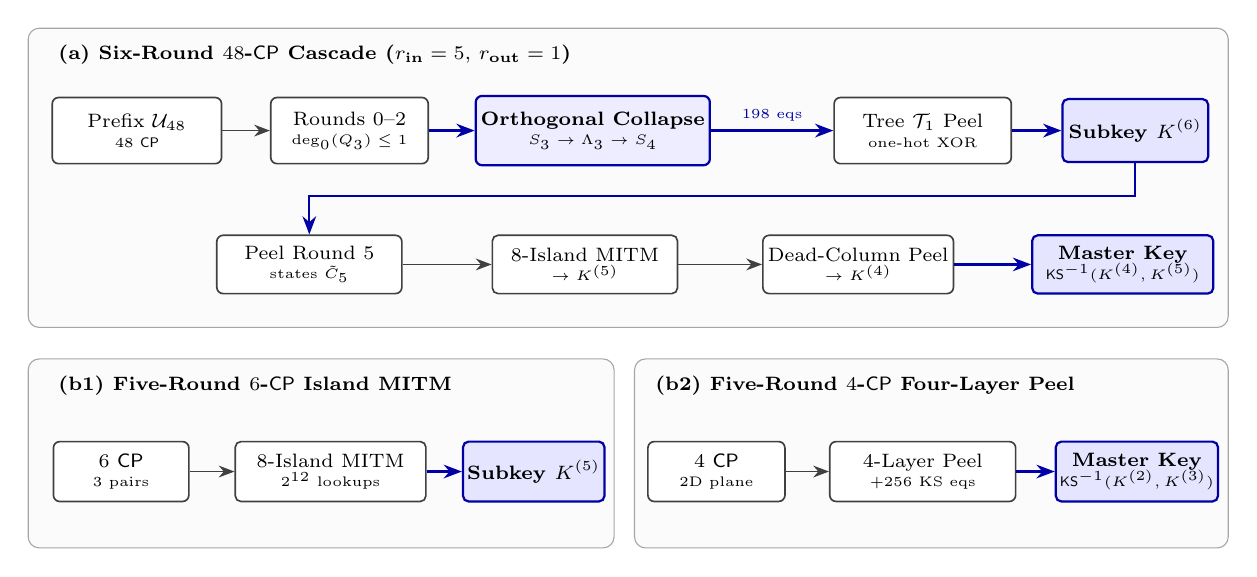
\begin{tikzpicture}[
    >=Stealth,
    stageb/.style={rectangle, draw=black!75, semithick, rounded corners=0.8mm, fill=white, minimum width=21.5mm, minimum height=8.4mm, inner sep=1.8pt, font=\scriptsize, align=center},
    collb/.style={rectangle, draw=blue!65!black, thick, rounded corners=0.8mm, fill=blue!7, minimum width=28.5mm, minimum height=8.8mm, inner sep=1.8pt, font=\scriptsize\bfseries, align=center},
    peelb/.style={rectangle, draw=black!75, semithick, rounded corners=0.8mm, fill=white, minimum width=22.5mm, minimum height=8.4mm, inner sep=1.8pt, font=\scriptsize, align=center},
    keyb/.style={rectangle, draw=blue!65!black, thick, rounded corners=0.7mm, fill=blue!10, minimum width=19.2mm, minimum height=8.0mm, inner sep=1.5pt, font=\scriptsize\bfseries, align=center},
    mitmb/.style={rectangle, draw=black!75, semithick, rounded corners=0.7mm, fill=white, minimum width=23.5mm, minimum height=7.8mm, inner sep=1.8pt, font=\scriptsize, align=center},
    tlbl/.style={font=\tiny, inner sep=1pt},
    wire/.style={->, semithick, draw=black!75},
    redwire/.style={->, thick, draw=blue!65!black},
    okwire/.style={->, thick, draw=blue!65!black}
]

% ================= PANEL (a): 6-ROUND 48-CP COLLAPSE & MASTER-KEY CASCADE =================
\begin{scope}[on background layer]
    \draw[rounded corners=1.4mm, draw=black!35, fill=gray!3] (-0.12, -1.65) rectangle (15.12, 2.15);
\end{scope}
\node[font=\scriptsize\bfseries, anchor=north west] at (0.14, 2.06) {(a) Six-Round $48\text{-}\CP$ Cascade ($r_{\text{in}} = 5,\, r_{\text{out}} = 1$)};

\node[stageb, minimum width=21.5mm] (u48) at (1.26, 0.85) {Prefix $\mathcal{U}_{48}$\\[-1pt]{\tiny $48~\CP$}};
\node[stageb, minimum width=20.0mm] (r02) at (3.96, 0.85) {Rounds $0\text{--}2$\\[-1pt]{\tiny $\deg_0(Q_3) \le 1$}};
\node[collb,  minimum width=29.0mm] (col) at (7.05, 0.85) {Orthogonal Collapse\\[-1pt]{\tiny $S_3 \to \Lambda_3 \to S_4$}};
\node[peelb,  minimum width=22.5mm] (p6)  at (11.24, 0.85) {Tree $\mathcal{T}_1$ Peel\\[-1pt]{\tiny one-hot XOR}};
\node[keyb,   minimum width=18.5mm] (k6)  at (13.94, 0.85) {Subkey $K^{(6)}$};

\draw[wire] (u48) -- (r02);
\draw[redwire] (r02) -- (col);
\draw[redwire] (col) -- node[tlbl, above=2.0pt, text=blue!65!black] {$198$ eqs} (p6);
\draw[okwire] (p6) -- (k6);

\node[peelb, minimum width=23.5mm, minimum height=7.4mm] (c5) at (3.45, -0.85) {Peel Round $5$\\[-1pt]{\tiny states $\tilde{C}_5$}};
\node[mitmb, minimum width=23.5mm, minimum height=7.4mm] (k5) at (6.95, -0.85) {$8$-Island MITM\\[-1pt]{\tiny $\to K^{(5)}$}};
\node[peelb, minimum width=23.5mm, minimum height=7.4mm] (k4) at (10.42, -0.85) {Dead-Column Peel\\[-1pt]{\tiny $\to K^{(4)}$}};
\node[keyb,  minimum width=23.0mm, minimum height=7.4mm] (mk6) at (13.78, -0.85) {Master Key\\[-1pt]{\tiny $\mathsf{KS}^{-1}(K^{(4)},K^{(5)})$}};

\draw[okwire] (k6.south) -- (13.94, 0.02) -| (c5.north);
\draw[wire] (c5) -- (k5);
\draw[wire] (k5) -- (k4);
\draw[okwire] (k4) -- (mk6);

% ================= PANEL (b): 5-ROUND ULTRA-LOW-DATA REGIMES =================
\begin{scope}[yshift=-4.00cm]
    \draw[rounded corners=1.4mm, draw=black!35, fill=gray!3] (-0.12, -0.45) rectangle (7.32, 1.95);
    \node[font=\scriptsize\bfseries, anchor=north west] at (0.14, 1.86) {(b1) Five-Round $6\text{-}\CP$ Island MITM};

    \node[stageb, minimum width=17.2mm, minimum height=7.6mm] (b1p) at (1.06, 0.52) {$6~\CP$\\[-1pt]{\tiny $3$ pairs}};
    \node[mitmb,  minimum width=24.2mm, minimum height=7.6mm] (b1m) at (3.72, 0.52) {$8$-Island MITM\\[-1pt]{\tiny $2^{12}$ lookups}};
    \node[keyb,   minimum width=16.5mm, minimum height=7.6mm] (b1k) at (6.30, 0.52) {Subkey $K^{(5)}$};

    \draw[wire] (b1p) -- (b1m);
    \draw[okwire] (b1m) -- (b1k);

    \draw[rounded corners=1.4mm, draw=black!35, fill=gray!3] (7.58, -0.45) rectangle (15.12, 1.95);
    \node[font=\scriptsize\bfseries, anchor=north west] at (7.72, 1.86) {(b2) Five-Round $4\text{-}\CP$ Four-Layer Peel};

    \node[stageb, minimum width=17.4mm, minimum height=7.6mm] (b2p) at (8.62, 0.52) {$4~\CP$\\[-1pt]{\tiny $2$D plane}};
    \node[peelb,  minimum width=23.6mm, minimum height=7.6mm] (b2m) at (11.24, 0.52) {$4$-Layer Peel\\[-1pt]{\tiny $+ 256$ KS eqs}};
    \node[keyb,   minimum width=19.8mm, minimum height=7.6mm] (b2k) at (13.96, 0.52) {Master Key\\[-1pt]{\tiny $\mathsf{KS}^{-1}(K^{(2)},K^{(3)})$}};

    \draw[wire] (b2p) -- (b2m);
    \draw[okwire] (b2m) -- (b2k);
\end{scope}

\end{tikzpicture}
\caption{Depth-one ($r_{\text{out}} = 1$) key-recovery flows in $\OPTIC$. \textbf{(a)}~On $6$ rounds ($48~\CP$ prefix $\mathcal{U}_{48}$), Theorem~\ref{thm:orth-collapse} provides $198$ zero-sum equations that isolate $K^{(6)}$ and cascade through $K^{(5)}$ and $K^{(4)}$ on the \emph{same} $48$ ciphertexts (zero extra queries) to recover the $256$-bit master key in $2.4\text{ s}$. \textbf{(b1)}~$5$-round $6\text{-}\CP$ eight-island MITM ($11\text{ ms}$; $6.21~\CP$ mean with adaptive $4$-th pair). \textbf{(b2)}~$5$-round $4\text{-}\CP$ four-layer subspace peel coupled with $256$ Law~III key-schedule relations ($16.0\text{ s}$).}
\label{fig:aradi-attack}
\end{figure}

\paragraph{3. Six-Round $48\text{-}\CP$ One-Hot XOR Solving and Three-Layer Master-Key Cascade ($2.4\text{ s}$).}
On $6$-round $\ARADI$ ($C = \Lambda_1(\pi(Q_5 \oplus K^{(5)})) \oplus K^{(6)}$), we compute $T^{(t)} = \Lambda_1(C^{(t)})$ ($0 \le t < 48$) on $\mathcal{U}_{48}$ and write $Y^{(t)}(\lambda) = \pi^{-1}(T^{(t)} \oplus \lambda) = Q_5(P^{(t)}) \oplus K^{(5)}$ for $\lambda = \Lambda_1(K^{(6)})$. Because $\Lambda_0(Y^{(t)}) = Z_4(P^{(t)}) \oplus \Lambda_0(K^{(5)})$ and every certified point mask $S \subset \{0,\dots,47\}$ from Regime~II has even Hamming weight, each of the $198$ island identities takes the exact depth-$1$ leaf-sum form
\begin{equation}
\label{eq:6r-xor}
\bigoplus_{t \in S} \bigoplus_{c \in \mathcal{C}_g} Y_{r, c}^{(t)}(\lambda_{\uparrow c}) = 0 \qquad (r \in \{x, z\}),
\end{equation}
where $\mathcal{C}_g = \supp(\mathbf{1}_{G_g}^\top L_0) = G_g \cup G_{(g+1)\bmod 8} \cup G_{(g+5)\bmod 8}$ spans $|\mathcal{C}_g| = 12$ leaves ($3$ islands). Encoding~\eqref{eq:6r-xor} as $198$ sparse XOR clauses over the $512$ one-hot variables $x_{c,v} = [\lambda_{\uparrow c} = v]$ alongside $32$ column one-hot constraints ($198 > 128$ bits of filtering on $\{0,1\}^{512}$) isolates $K^{(6)} = \Lambda_1(\lambda)$ in $2.2\text{ s}$ median via CryptoMiniSat~\cite{CMS}. Peeling Round~$5$ on the \emph{same} $48$ ciphertexts yields $\tilde{C}_5^{(0\dots 47)}$, from which our $2^{12}$ eight-island MITM recovers $K^{(5)}$ in $71\text{ ms}$ and a deterministic $2$-round dead-column peel recovers $K^{(4)}$ in $108\text{ ms}$. Law~III.1 ($\mathsf{KS}^{-1}(K^{(4)}, K^{(5)}, 4)$) then outputs the full $256$-bit master key in $2.4\text{ s}$ median ($32\times$ less data than~\cite[Footnote~4]{DG25}; Algorithm~2).

\begin{figure}[t]
\centering
\small
\begin{tabular}{@{}p{0.97\textwidth}@{}}
\toprule
\textbf{Algorithm 2:} $\OPTIC$ Instantiation at $(d{=}6, r_{\text{in}}{=}5, r_{\text{out}}{=}1)$: Zero-Sampling $6$-Round $48\text{-}\CP$ Master-Key Recovery \\
\midrule
\textbf{Module I Offline Analytical Certificate (runs once in $\approx 5\text{ ms}$, $0$ key samples):} \\
\hspace*{1.2em} \textbf{1.} Propagate exact ANF monomial supports of $\mathcal{D}_6$ in~\eqref{eq:cube48} through $3$ rounds ($Q_0 \to Q_3$) via~\eqref{eq:sbox-anf}--\eqref{eq:Lj}. \\
\hspace*{1.2em} \textbf{2.} For each island $G_g$ ($0 \le g \le 7$), form the degree-$3$ super-S-box monomial unions~\eqref{eq:collapse} and extract the $\Ftwo$-nullspace on $\mathcal{U}_{48}$, obtaining $99 + 99 = 198$ universal zero-sum triples $(r, \mathcal{C}_g, S)$. \\[3pt]
\midrule
\textbf{Modules II \& III Online Key Recovery from $48$ Chosen Plaintexts $\mathcal{U}_{48}$:} \\
\hspace*{1.2em} \textbf{1.} Query $C^{(t)} \leftarrow \mathsf{ARADI}_6(P^{(t)})$ for $t = 0, \dots, 47$, and compute $T^{(t)} \leftarrow \Lambda_1(C^{(t)})$. \\
\hspace*{1.2em} \textbf{2.} \textbf{Layer 1 ($K^{(6)}$):} Encode the $32$ one-hot column groups on $(x_{c,v})_{0 \le c < 32,\, 0 \le v < 16}$ and the $198$ XOR clauses~\eqref{eq:6r-xor}; solve via CNF-XOR propagation to obtain $K^{(6)} \leftarrow \Lambda_1(\lambda)$. \\
\hspace*{1.2em} \textbf{3.} \textbf{Layer 2 ($K^{(5)}$ in $\approx 71\text{ ms}$):} Peel Round~$5$ on all $48$ ciphertexts: $\tilde{C}_5^{(t)} \leftarrow \pi^{-1}(\Lambda_1(C^{(t)} \oplus K^{(6)})) = Q_5(P^{(t)}) \oplus K^{(5)}$. Apply the $2^{12}$ eight-island MITM join~\eqref{eq:mitm-join} across the $128$ single-column pairs inside $\mathcal{U}_{48}$ to recover $K^{(5)}$. \\
\hspace*{1.2em} \textbf{4.} \textbf{Layer 3 ($K^{(4)}$ \& Master Key in $\approx 108\text{ ms}$):} Peel Round~$4$: $\tilde{C}_4^{(t)} \leftarrow \pi^{-1}(\Lambda_0(\tilde{C}_5^{(t)} \oplus K^{(5)})) = Q_4(P^{(t)}) \oplus K^{(4)}$; recover $K^{(4)}$ from deterministic $2$-round dead-column equations ($\ge 23$ dead columns per pair across $\mathcal{U}_{48}$). \\
\hspace*{1.2em} \textbf{5.} \textbf{Module III Closure:} Compute $K_{\text{master}} \leftarrow \mathsf{KS}^{-1}(K^{(4)}, K^{(5)}, 4)$ via Algorithm~1 ($2m = 4$ even), verify $\mathsf{ARADI}_6(P^{(t)}, K_{\text{master}}) = C^{(t)}$ for all $0 \le t < 48$, and \textbf{return} $K_{\text{master}} \in \{0,1\}^{256}$. \\
\bottomrule
\end{tabular}
\end{figure}

\subsection{Depth-Two Peeling on Seven and Eight Rounds}
\label{subsec:depth2}

When $r_{\text{out}} = 2$, each subtree of $\mathcal{T}_2$ spans $3$ leaf nibbles ($12$ bits of $\lambda^{(R)}$) fed into a middle-layer inverse S-box $\pi^{-1}(\cdot \oplus \lambda^{(R-1)}_{\uparrow u})$ ($4$ bits), which we evaluate via two fast Walsh--Hadamard strategies:
\begin{enumerate}[leftmargin=1.8em]
    \item \textbf{Seven-Round Single-Subtree $2^{12}$ FHT Peel ($3{,}072~\CP$, $3.5\text{ s}$):} Instantiating Module~I with six shifted $9$D Regime~III cubes $B_2^{(s)} \cup \{z_{(5+s)\bmod 16}\}$ ($6 \times 512 = 3{,}072~\CP = 2^{11.58}~\CP$) provides $324$ ZeroSum bits on $Q_5$. Each balanced column of $Q_5$ depends on a single depth-$2$ subtree with $3$ leaves ($12$ bits of $\lambda^{(7)} = \Lambda_2(K^{(7)})$), which a $2^{12}$-point FHT (as in~\cite{TA14} and the $6$-round prototype of~\cite{DG25}) evaluates in $<1\text{ ms}$. Peeling Round~$6$ onto the $19$ balanced columns of $Z_4 = \Lambda_0(Q_5)$ recovers $K^{(6)}$, and Module~III ($\mathsf{KS}^{-1}(K^{(6)}, K^{(7)}, 6)$~\cite[Remark~5]{DG25}) outputs the $256$-bit master key in $3.5\text{ s}$ median on $1$ core ($>2^{20}\times$ less data than~\cite{BBGHP25}).
    \item \textbf{Eight-Round Root-Free $3$-Branch Additive-Split Bloom-MITM ($90{,}112~\CP$, $6.0\text{ s}$):} On $8$-round $\ARADI$, instantiating Module~I at the $4$ balanced columns $\{10, 18, 25, 31\}$ of $Z_5 = \Lambda_1(Q_6)$ under the $12$D Regime~III cube $B_3^{(s)}$ ($2^{12}~\CP$) \emph{stops prior to the root inverse S-box $S_5^{-1}$}. Because $\Lambda_1$ is linear, with $T_8 = \Lambda_3(C_8)$, $\lambda^{(8)} = \Lambda_3(K^{(8)})$, $\lambda^{(7)} = \Lambda_2(K^{(7)})$, and $\supp_b(L_1) = \{u_0, u_1, u_2\}$, the root-free tree $\mathcal{T}_{2.5}$ splits additively into three independent $16$-bit depth-$2$ subtrees:
    \[
    F_{u_0}\!\bigl(\lambda^{(7)}_{\uparrow u_0}, \lambda^{(8)}_{N(u_0)}\bigr) \;\oplus\;
    F_{u_1}\!\bigl(\lambda^{(7)}_{\uparrow u_1}, \lambda^{(8)}_{N(u_1)}\bigr) \;=\;
    F_{u_2}\!\bigl(\lambda^{(7)}_{\uparrow u_2}, \lambda^{(8)}_{N(u_2)}\bigr),
    \]
    where $N(u) = \supp_u(L_2)$ ($|N(u)| = 3$ leaves). We evaluate each $2^{16}$-entry subtree table via FHT on $11$ cubes at $s = 0$ and $11$ at $s = 8$ ($90{,}112~\CP = 2^{16.46}~\CP$, $1.44\text{ MB}$ of ciphertexts, $<20\text{ MB}$ total RAM). Indexing $F_{u_2}$ in a $2\text{ MB}$ L3-resident Bloom filter then solves $b = 25$ in $2^{32}$ lookups, cascades through the remaining subtrees, and closes via Module~III ($\mathsf{KS}^{-1}(K^{(6)}, K^{(7)}, 6)$) in $6.0\text{ s}$ mean ($5.7\text{ s}$ median) on $1$ core.
\end{enumerate}

\subsection{Depth-Three Streaming WHT on Nine Rounds}
\label{subsec:depth3}
\label{subsec:9r}

For $9$-round $\ARADI$ ($C = Q_9 \oplus K^{(9)}$ at $r_0 = 0$), our $16$D Regime~III distinguisher $B_4^{(s)}$ on $Q_6$ sets the tree depth to $r_{\text{out}} = 3$ (Rounds $8, 7, 6$, using $\Lambda_0, \Lambda_3, \Lambda_2$). With $T_9 = \Lambda_0(C)$ and transformed round keys $\kappa = \Lambda_0(K^{(9)})$, $\gamma = \Lambda_3(K^{(8)})$, and $g = \Lambda_2(K^{(7)})$, the depth-$3$ ternary tree $\mathcal{T}_{3, u}$ rooted at balanced column $u = 16 + ((9 + s)\bmod 16)$ of $Q_6 = Z_6 \oplus K^{(6)}$ reads
\begin{equation}
\label{eq:9r-peel}
\begin{aligned}
Z_{8,\uparrow d} &= \pi^{-1}(T_{9,\uparrow d} \oplus \kappa_{\uparrow d}), &\qquad
M_e &= \bigoplus_{d \in \supp_e(L_3)} Z_{8,\uparrow d}, \\
V_u &= \bigoplus_{e \in E(u)} \pi^{-1}(M_e \oplus \gamma_{\uparrow e}), &\qquad
Z_{6,\uparrow u} &= \pi^{-1}(V_u \oplus g_{\uparrow u}),
\end{aligned}
\end{equation}
where $E(u) = \supp_u(L_2)$ has $|E(u)| = 3$ internal nodes and $D(u) = \bigcup_{e \in E(u)} \supp_e(L_3)$ has $|D(u)| = 9$ disjoint leaves for \emph{every} $u \in \{0,\dots,31\}$ ($9 \times 4 + 3 \times 4 + 4 = 52$ branch key bits).

\paragraph{Streaming Joint-Histogram WHT Kernel ($\mathsf{JM\text{-}WHT}$).}
Unlike the root-free $8$-round tree, the root $\pi^{-1}(V_u \oplus g_{\uparrow u})$ in~\eqref{eq:9r-peel} nonlinearly couples the three subtrees $e_1, e_2, e_3 \in E(u)$. When $d \ge 113 \gg 36$, the bottom-up $3$-round partial-sum FHT of~\cite[$\S$3.2, Algorithm~3]{DG25} must first tabulate a $2^{36}$-entry leaf array ($2^{41}$ bits $= 256\text{ GB}$ in $32$-bit words) before reducing to the three middle nodes. Because our Regime~III cube has size $|\mathcal{C}| = 2^{16} \ll 2^{36}$, we bypass the leaf FHT stages entirely. Fixing only the \emph{unrecovered} leaf nibbles of $\kappa_{D(u)}$ in an outer loop, we stream $\mathcal{C}$ in $2^{16}$ steps directly into the $4{,}096$-byte $12$-bit \emph{joint} parity histogram $\mathsf{JM}[m_1, m_2, m_3] = \#\{P \in \mathcal{C} : (M_{e_1}, M_{e_2}, M_{e_3})(P) = (m_1, m_2, m_3)\} \bmod 2$. We then evaluate the middle-to-root parity-distribution convolution of~\cite{DGK24,DG25} in the Walsh character basis $H_\xi(m_1,m_2,m_3) = (-1)^{\langle \xi,\, \pi^{-1}(m_1)\oplus\pi^{-1}(m_2)\oplus\pi^{-1}(m_3)\rangle}$ ($\xi \in \Ftwo^4$). This yields $\Phi_\gamma[z] = \#\{P \in \mathcal{C} : V_u(P) = z\} \bmod 2$ simultaneously for all $2^{12}$ middle keys $\gamma_{E(u)}$ via $16$ size-$2^{12}$ WHTs.
\begin{equation}
\label{eq:9r-wht}
\begin{aligned}
\widehat{N}_\gamma[\xi] &= 2^{-12}\,\mathsf{WHT}_{12}\!\bigl(\widehat{\mathsf{JM}} \odot \widehat{H}_\xi\bigr)[\gamma], \qquad
\Phi_\gamma = \bigl(2^{-4}\,\mathsf{WHT}_4(\widehat{N}_\gamma)\bigr) \bmod 2, \\
\mathcal{Z}_u(\gamma, g) &= \bigoplus_{z : \Phi_\gamma[z] = 1} \pi^{-1}(z \oplus g) = 0.
\end{aligned}
\end{equation}
Chaining shifts $s = 0, \dots, 15$ sequentially ($u = 25,\dots,31, 16,\dots,24$), already-recovered $\kappa$ and $\gamma$ columns prune subsequent trees. Shift~$0$ searches $36$ $\kappa$-bits ($13$ cubes), shift~$1$ searches $20$ new $\kappa$-bits ($9$ cubes), shifts~$2$--$5$ search $16$ bits ($8$ cubes each), shift~$6$ searches $8$ bits ($6$ cubes), and shifts~$7$--$15$ search $0$ new $\kappa$-bits ($2$--$3$ cubes each, $20$ cubes total). This schedule requires $80$ cubes ($D = 80 \cdot 2^{16} = 2^{22.32}~\CP$), $T = 2^{54.77}$ FHT butterflies ($= 2^{57.52}$ $64$-bit word ops $\approx 2^{45.33}$ $9$-round encryptions; reducible to $2^{56.1}$ word ops via $3$-group character MITM), and $M = 2^{25.16}$ bits ($4.7\text{ MB}$, $>5 \times 10^4\times$ smaller than $256\text{ GB}$). Across all $16$ shifts, the recovered nibbles cover $32/32$ columns of both $\kappa = \Lambda_0(K^{(9)})$ and $\gamma = \Lambda_3(K^{(8)})$ ($\Ftwo$ rank $\rho = 256$, residual $2^0$), and Module~III ($\mathsf{KS}^{-1}(K^{(8)}, K^{(9)}, 8)$) outputs the unique $256$-bit master key in $O(1)$ (Algorithm~3).

\begin{figure}[t]
\centering
\small
\begin{tabular}{@{}p{0.97\textwidth}@{}}
\toprule
\textbf{Algorithm 3:} $\OPTIC$ Instantiation at $(d{=}16, r_{\text{in}}{=}6, r_{\text{out}}{=}3)$: $9$-Round Streaming $\mathsf{JM\text{-}WHT}$ Master-Key Recovery \\
\midrule
\textbf{Offline Precomputation ($< 1\text{ ms}$, $1.1\text{ MB}$):} \\
\hspace*{1.2em} \textbf{1.} For each $\xi \in \Ftwo^4$, tabulate $H_\xi[m_1, m_2, m_3] = (-1)^{\langle \xi,\, \pi^{-1}(m_1)\oplus\pi^{-1}(m_2)\oplus\pi^{-1}(m_3)\rangle}$ and $\widehat{H}_\xi \leftarrow \mathsf{WHT}_{12}(H_\xi)$. \\[3pt]
\midrule
\textbf{Modules II \& III Online Recovery ($D = 2^{22.32}~\CP$, $M = 4.7\text{ MB}$, $\rho = 256$):} \\
\hspace*{1.2em} \textbf{1.} \textbf{for} shift $s = 0$ \textbf{to} $15$ ($u = 16 + ((9 + s)\bmod 16)$, $E = \supp_u(L_2)$, $D = \bigcup_{e \in E}\supp_e(L_3)$) \textbf{do} \\
\hspace*{2.6em} Query $m_s$ translates of $B_4^{(s)}$ ($2^{16}~\CP$ each) and extract $T_{9,\uparrow d} = \Lambda_0(C)_{\uparrow d}$ for $d \in D$. \\
\hspace*{2.6em} Enumerate only unrecovered nibbles of $\kappa_D$ (fixing all $\kappa_d$ already recovered in shifts $< s$): \\
\hspace*{4.0em} Build $\mathsf{JM}$ on cube~$0$, compute $\widehat{\mathsf{JM}} \leftarrow \mathsf{WHT}_{12}(\mathsf{JM})$, evaluate $\Phi_\gamma$ via~\eqref{eq:9r-wht} on consistent $\gamma_E$, \\
\hspace*{4.0em} collect $(\gamma_E, g_u)$ with $\mathcal{Z}_u(\gamma_E, g_u) = 0$, and filter survivors across cubes $1, \dots, m_s{-}1$. \\
\hspace*{2.6em} Commit unique $\kappa_D$; propagate cross-shift $\gamma_E$ consistency (each $\gamma$ column appears in $3$ shifts). \\
\hspace*{1.2em} \textbf{2.} \textbf{Module III Closure:} Reconstruct $K^{(9)} \leftarrow \Lambda_0(\kappa)$ and $K^{(8)} \leftarrow \Lambda_3(\gamma)$, and \textbf{return} $K_{\text{master}} \leftarrow \mathsf{KS}^{-1}(K^{(8)}, K^{(9)}, 8)$. \\
\bottomrule
\end{tabular}
\end{figure}

\subsection{Multi-Tree List Joins on Ten to Twelve Rounds}
\label{subsec:depth4}
\label{subsec:10r-12r}

For $R \in \{10, 11, 12\}$ at unmodified offset $r_0 = 0$, coupling our $16$D Regime~III distinguisher ($r_{\text{in}} = 6$) with a depth-$4$ ternary tree ($r_{\text{out}} = 4$, leaf widths $1, 3, 9, 23 \implies 36$ tree nodes $= 144$ branch bits) yields an ultra-low-data $10$-round all-key corner of $(D = 2^{22.00}~\CP, T = 2^{137.21}\text{ enc.}, M = 2^{25.0}\text{ bits}, \rho = 256)$---$2^{96}\times$ less data than any prior $10$-round attack. In the high-data Regime~IV ($r_{\text{in}} \in \{7, 8\}$, $d \in \{113, 116, 124\}$), introducing four targeted refinements into the multi-tree FHT and greedy column-overlap list-join framework of Dunkelman and Ghosh~\cite{DG25} improves both data and time upon~\cite{DG25} across \emph{all three} of $10$, $11$, and $12$ rounds under identical packed-arithmetic accounting:
\begin{enumerate}[leftmargin=1.8em]
    \item \textbf{Regime~IV $d = 113$ Toffoli Pullback on $10$ Rounds ($r_{\text{in}} = 7, r_{\text{out}} = 3$):} Replacing the $d = 116$ cube of~\cite[$\S$3.2]{DG25} with the $d = 113$ $e_x \oplus e_z$ Toffoli distinguisher~\cite{BRRT25} (Section~\ref{subsec:regime4}, $m = 16$ cubes, $16$-bit filter/column, $13$ trees) reproduces the list trajectory of~\cite[Table~7]{DG25} ($\max_t |L_t| = 2^{40}$, $M = 2^{46.17}\text{ bits}$) at $D = 2^{117.0}~\CP, T = 2^{117.0}\text{ enc.}$, beating~\cite[$\S$3.2]{DG25} $(2^{118}, 2^{118}, 2^{48}\text{ bits})$ in all three metrics. Using $m = 8$ cubes ($24$ trees under the greedy overlap order of~\cite{DG25}, $\rho = 256$, $\max_t |L_t| = 2^{102}$, join $2^{103.61} \ll 2^{116}$) achieves $D = 2^{116.0}~\CP, T = 2^{116.0}\text{ enc.}, M = 2^{109.89}\text{ bits}$ ($4\times$ lower data and time).
    \item \textbf{$O(1)$ Root Parity-Pattern Lookup Table:} In~\cite[Algorithm~3]{DG25}, after reducing the $K$-node ternary tree ($K = \sum_{i=r_{\text{in}}+1}^{R} |T_i(c)|$) to the $4$-bit parity pattern $B[0\dots 15]$ entering the root, the final loop evaluates $\bigoplus_{b: B[b]=1} \pi^{-1}(u^{(r_{\text{in}}+1)}_{\uparrow c} \oplus b)$ over all $16$ root keys ($2^{G_{\text{fin}} + 5.04}$ packed ops). Precomputing a $2^{16} \times 16$ lookup table ($2^{22}$ bits) replaces this loop by an $O(1)$ lookup ($2^{G_{\text{fin}}}$ ops), lowering depth-$3$ packed peel cost to $2^{54.75}$ and depth-$4$ ($|T_R(c)|=22$) packed cost to $2^{142.75}$.
    \item \textbf{Tight $m = 3$ Lai-Coset Sizing and $L_t$-Guided Leaf Pruning on $11$ Rounds:} Auditing intermediate hash-join list sizes $|L_t|$ at every step~$t$ under the greedy column-overlap order of~\cite{DG25} shows that $m = 2$ cubes ($6$-bit Lai coset filter~\cite{Lai94},~\cite[Table~5]{DG25}) on $11$ rounds ($8$R $d = 124$~\cite{BRRT25}) causes $|L_t|$ to peak at $2^{136.9} \gg 2^{125}$. By contrast, $m = 3$ cubes ($10$-bit filter, $19$ trees) already bounds $\max_t |L_t| = 2^{92}$ ($T_{\text{join}} = 2^{93.2} \ll D$). This yields $D = 3 \cdot 2^{124} = 2^{125.58}~\CP, T = 2^{125.58}\text{ enc.}, M = 2^{99.58}\text{ bits}$, beating $m = 4$ in~\cite[$\S$3.3]{DG25} $(2^{126}, 2^{126})$ in $D$ and $T$ at higher list-join memory vs.\ $2^{48}\text{ bits}$. On the low-data $7$R $d = 116$~\cite{DG25} branch ($4$ depth-$4$ trees $[0, 8, 23, 31]$), after Step~$3$ the surviving list has $|L_3| = 2^{84}$ ($m=7$, peak $\max_t |L_t| = 2^{112}$ at Step~$2$), strictly smaller than $2^{88}$ leaf guesses of $u^{(11)}$ ($0$ new $u^{(11)}$ bits at Step~$4$). Restricting Step~$4$'s outer FHT to $u^{(11)}$ projections present in $L_3$ eliminates Step~$4$'s $2^{145.6}$ cost completely, giving $D = 7 \cdot 2^{116} = 2^{118.81}~\CP, T = 2^{147.17}\text{ packed ops}, M = 2^{119.46}\text{ bits}$ (beating~\cite[$\S$3.4]{DG25} $(2^{119}, 2^{147.76})$ in $D$ and $T$, vs.\ $M = 2^{107.1}\text{ bits}$).
    \item \textbf{Law~II.3 Lower-Half $|T_{12}(c)| = 22$ Narrow-Tree Selection on $12$ Rounds:} In~\cite[$\S$3.5, Table~11]{DG25}, $4$ of the $8$ chosen roots $\{19, 30, 25, 20\}$ lie in the upper half $\{16\dots 31\}$ where the depth-$4$ leaf cone has width $|T_{12}(c)| = 23$ ($2^{146.76}$ packed ops/cube), dominating their $T = 2^{151.80}$ total. By Law~II.3, \emph{all $16$ lower-half roots $\{0\dots 15\}$ satisfy $|T_{12}(c)| = 22$} ($16\times$ cheaper per tree) and already span full master-key rank $\rho = 256$. We obtain two complementary all-key $12$-round tradeoffs. First, (a)~using one upper-half overlap anchor ($c = 19$ at Step~$2$ to cap $\max_t |L_t| = 2^{116}$) followed by lower-half trees $[0, 19, 11, 6, 1, 12, 7]$ with $L_t$-guided pruning at $m = 7$ achieves $D = 2^{126.81}~\CP, T = 2^{149.88}\text{ packed ops}, M = 2^{123.49}\text{ bits}$ ($\rho = 256$, $M < 2^{128}$, strictly beating~\cite[$\S$3.5]{DG25} in both $T$ [$3.8\times$] and $M$ at equal $D$). Second, (b)~using $m = 6$ cubes on pure lower-half trees $[0, 5, 10, 11, 6]$ achieves $D = 6 \cdot 2^{124} = 2^{126.58}~\CP, T = 2^{148.62}\text{ packed ops} \approx 2^{141}\text{ enc.}, M = 2^{153.81}\text{ bits}$ ($9.1\times$ faster than~\cite[$\S$3.5]{DG25} at lower $D$, and $>2^{48}\times$ faster than the non-heuristic $T = 2^{197}$ weak-key attack of~\cite[Table~1]{BNS26}).
\end{enumerate}

\section{Experiments and Discussion}
\label{sec:experiments}

\subsection{Experimental Verification}
\label{subsec:exp-summary}

We implemented all distinguishers, key-recovery solvers, and complexity auditors in portable single-core Python~3 and C99, first verifying bit-exact compliance against all $21$ official $\ARADI$ test vectors and round-key schedules~\cite{GMW24}. Table~\ref{tab:experiments} summarizes our empirical results across three blocks:
\begin{enumerate}[leftmargin=1.8em]
    \item \textbf{Algebraic Certificates and Distinguishers ($5$--$6$ Rounds):} Exhaustive $16$-bit binary M\"{o}bius evaluation verifies the degree-$3$ super-S-box spectrum (Proposition~\ref{prop:supersbox-spectrum}) in $1.4\text{ s}$, while symbolic ANF propagation derives all $198$ universal $5$-round zero-sum equations on the $48\text{-}\CP$ prefix $\mathcal{U}_{48}$ in $5\text{ ms}$ ($0$ violations across $9{,}900$ random key trials). On $6$ rounds, live evaluation of the $2^{16}\text{-}\CP$ colliding cube $B_4^{(0)}$ confirms full $128$D inner balance on $Q_5$ and the $42$D balanced linear-mask null space on $Q_6$ across $640$ key trials ($384$ master keys and $256$ independent round-key tuples, $0.03\text{ s}$ per key).
    \item \textbf{End-to-End Key Recovery ($5$--$8$ Rounds):} Unassisted single-core solvers achieve $100\%$ recovery across all random SplitMix64 trials within $<20\text{ MB}$ peak RAM. On $5$ rounds, the $8$-island MITM recovers $128$-bit $K^{(5)}$ from $6~\CP$ ($6.21~\CP$ mean with an adaptive $4$-th pair) in $11\text{ ms}$ median ($200/200$ trials), and the $4$-layer CNF-XOR peel recovers the full $256$-bit master key from $4~\CP$ in $16.0\text{ s}$ median ($10/10$ trials). On $6$, $7$, and $8$ rounds, our $3$-layer cascade ($48~\CP$), single-subtree $2^{12}$ FHT ($3{,}072~\CP$), and root-free $3$-branch FHT with a $2\text{ MB}$ Bloom filter ($90{,}112~\CP$) recover the full $256$-bit master key in $2.4\text{ s}$ median, $3.5\text{ s}$ median, and $6.0\text{ s}$ mean, respectively ($10/10$ trials each).
    \item \textbf{Higher-Round Kernel and Complexity Verification ($9$--$12$ Rounds):} Because full $9$-round recovery has complexity $T = 2^{54.77}$ FHT butterflies ($2^{36}$ outer leaf guesses of $\kappa$), we verify a single iteration of the inner $16$-shift streaming $\mathsf{JM\text{-}WHT}$ kernel~\eqref{eq:9r-wht} across all $2^{16}$ $(\gamma_E, g_u)$ candidates per shift, cross-shift $K^{(8)}$ propagation, and $\mathsf{KS}^{-1}(K^{(8)}, K^{(9)}, 8)$ closure under a fixed outer $\kappa$. For $9$--$12$ rounds, exact $\Ftwo$ symbolic rank and progressive list-join auditors ($0.3\text{ s}$ total) verify the subkey-span rank $\rho$ and peak intermediate list sizes $\max_t |L_t|$ underlying all $(D, T, M)$ bounds in Sections~\ref{subsec:depth3}--\ref{subsec:depth4}.
\end{enumerate}

\begin{table}[t!]
\centering
\caption{Single-core experimental verification of $\OPTIC$ across $5$- to $8$-round unmodified $\ARADI$ ($r_0 = 0$; $100\%$ success across all trials). ``Data'' is in chosen plaintexts ($\CP$).}
\label{tab:experiments}
\footnotesize
\setlength{\tabcolsep}{6.0pt}
\renewcommand{\arraystretch}{1.06}
\begin{tabular}{@{}cllrrr@{}}
\toprule
\textbf{Rds} & \textbf{Experiment} & \textbf{Verified Target} & \textbf{Data} & \textbf{Trials} & \textbf{Runtime} \\
\midrule
$5$ & Orthogonal-island zero-sum (\S\ref{subsec:regime2})      & $198$ zero-sum eqs    & $48$             & $9{,}900$ & $5\text{ ms}$ \\
$5$ & $8$-island MITM (\S\ref{subsec:depth1})                  & $128$-bit $K^{(5)}$   & $6^{\mathrm{a}}$ & $200$     & $11\text{ ms}$ \\
$5$ & $4$-layer CNF-XOR peel (\S\ref{subsec:depth1})           & $256$-bit MK          & $4$              & $10$      & $16.0\text{ s}$ \\
$6$ & Colliding-cube distinguisher (\S\ref{subsec:regime3})    & $42$D $Q_6$ nullspace & $2^{16}$         & $640$     & $0.03\text{ s}$ \\
$6$ & One-hot XOR + $3$-layer cascade (\S\ref{subsec:depth1})   & $256$-bit MK          & $48$             & $10$      & $2.4\text{ s}$ \\
$7$ & Single-subtree $2^{12}$ FHT (\S\ref{subsec:depth2})      & $256$-bit MK          & $3{,}072$        & $10$      & $3.5\text{ s}$ \\
$8$ & Root-free $3$-branch FHT + Bloom (\S\ref{subsec:depth2}) & $256$-bit MK          & $90{,}112$       & $10$      & $6.0\text{ s}$ \\
\bottomrule
\addlinespace[2pt]
\multicolumn{6}{@{}l@{}}{\scriptsize $^{\mathrm{a}}$$6.21~\CP$ mean with adaptive $4$-th pair.}
\end{tabular}
\end{table}

\subsection{Comparison with Quasidifferential Cryptanalysis}
\label{subsec:tosc-comparison}

Comparing $\OPTIC$ against the quasidifferential analysis of Beyne, Neyt, and Sajjad~\cite{BNS26} (\emph{ToSC 2026(3)}) highlights both the complementary tradeoffs across $5$--$14$ rounds and deep algebraic connections between the two paradigms:
\begin{enumerate}[leftmargin=1.8em]
    \item \textbf{All-Key Determinism ($100\%$ of $2^{256}$ Keys) vs.\ Weak-Key Differential Collapse ($5$--$12$ Rounds):}
    In~\cite{BNS26}, every differential characteristic with $R \ge 5$ rounds imposes linear constraints on the round keys via quasidifferential trails. Their $5$-round characteristic~\cite[Example~1, pp.~7--8]{BNS26} holds with probability $2^{-42}$ only on a $2^{-8}$ weak-key fraction (and zero otherwise), while their corrected $6$-round characteristic~\cite[Remark~1 and Appendix~A]{BNS26} has key-averaged probability $p_{\mathrm{avg}} = 2^{-82}$ (and Bellini et al.~\cite[Table~4]{BFG24}, reproduced in~\cite[Table~3]{BNS26}, report key-averaged characteristic bounds $p_{\mathrm{avg}} = 2^{-106}$, $2^{-122}$, and $2^{-137}$ for $7$, $8$, and $9$ rounds without fixed-key guarantees). Above $5$ rounds, Beyne et al.\ evaluate fixed-key differential probabilities only on $9$ rounds: for the Round-$0$ differential of~\cite{BFG24}, they obtain $2^{-109}$ on $3 \cdot 2^{256-28}$ keys and $2^{-106.678}$ on $2^{256-28}$ keys ($2^{-26}$ of the key space in total)~\cite[$\S$3.3]{BNS26}, and for two shifted-round $9$-round differentials they obtain $2^{-107.678}$ for a $2^{-38}$ fraction of keys and $2^{-119}$ for a $2^{-39}$ fraction of keys~\cite[$\S$5.2--5.3]{BNS26}. Likewise, their $12$-round key-recovery attack~\cite[$\S$6.1, Table~1]{BNS26} succeeds only for $2^{218}$ weak keys ($2^{-38}$ fraction) in time $T = 2^{196.68} \approx 2^{197}$ ($D = 2^{108.68}~\CP$, $M = 2^{36}$; or $T = 2^{117}$, $D = 2^{111.38}~\CP$, $M = 2^{82.38}$ under a binomial randomization heuristic with $63\%$ success on the $2^{-38}$ weak-key subset). Within its $2^{-38}$ weak-key class,~\cite[$\S$6.1]{BNS26} uses $2^{17.9}\times$ less data ($2^{108.68}$ vs.\ $2^{126.58}~\CP$) and lower memory ($2^{36}$ states vs.\ $2^{123.49}$ or $2^{153.81}$ bits) than our $12$-round integral attacks, and extends to $14$ rounds on $2^{-39}$ weak keys. Conversely, every Module~I identity in $\OPTIC$ holds \emph{deterministically with probability~$1$ for all $2^{256}$ master keys}. On $5$ and $6$ rounds we recover the full $256$-bit master key from $4~\CP$ ($16.0\text{ s}$) and $48~\CP$ ($2.4\text{ s}$). On $6$ rounds our $2^{16}\text{-}\CP$ distinguisher requires $2^{66}\times$ less data than~\cite[Appendix~A]{BNS26}, and on $7$--$9$ rounds we achieve full all-key recovery where~\cite{BNS26} gives no key recovery. On $12$ rounds we trade higher data and memory to expand the valid key space by $2^{38}\times$ while running $>2^{48}\times$ faster ($T = 2^{148.62}$ packed ops $\approx 2^{141}$ enc.) than the non-heuristic $T = 2^{197}$ attack of~\cite[Table~1]{BNS26}.
    \item \textbf{Unified Algebraic Origin of Half-Word Cone Asymmetry (Law~II.3 vs.~\cite[Table~5]{BNS26}):}
    In~\cite[$\S$5.1, Table~5]{BNS26}, Beyne et al.\ observed empirically via code search that extending a $1$-column distinguisher-output difference across $2$ or $3$ outer key-recovery rounds requires guessing fewer subkey columns when the active column lies in the ``left'' $16$-bit half (our upper half $u$, MSB columns $0\dots 15$) than in the ``right'' $16$-bit half (our lower half $l$, MSB columns $16\dots 31$). In particular, $|K_{\text{out}}| = 16$ vs.\ $18$ columns at $2$ rounds and $39$ vs.\ $43$ columns at $3$ rounds ($16$-bit difference). Law~II.3 explains both their observation and our $12$-round $|T_{12}(c)| = 22$ vs.\ $23$ leaf-cone split from a single matrix identity: for $j \in \{0,1,2\}$, $b_j + c_j \not\equiv 0 \pmod{16}$, so $L_j^\top \neq L_j$. In~\cite{BNS26}, differences propagate through $L_j$ while quasidifferential masks propagate through $L_j^{-\top} = L_j^\top$. In our depth-$4$ ternary tree $\mathcal{T}_4$, backward cones propagate through $L_0 \to L_1 \to L_2 \to L_3$, making lower-half roots $c \in \{0,\dots,15\}$ strictly narrower ($22$ leaves, $35$ total cone columns) than upper-half roots ($23$ leaves, $36$ total cone columns).
    \item \textbf{Exact Rank Audit of the $14$-Round Weak-Key Attack in~\cite[$\S$6.2]{BNS26}:}
    In their $14$-round weak-key attack ($2 + 9 + 3$ rounds on $2^{217}$ weak keys, $\dim W = 39$), Beyne et al.~\cite[Tables~11--12, p.~19]{BNS26} guess $16$ columns ($64$ bits) of $K_{\text{in}} \subset K^{(0)} \times L_0(K^{(1)})$ and $41$ columns ($164$ bits) of $K_{\text{out}} \subset L_1^{-1}(K^{(14)}) \times L_0^{-1}(K^{(13)}) \times L_3^{-1}(K^{(12)})$. Auditing their column sets under the exact MSB-first column bijection $b = 31 - c_{\text{MSB}}$ against Algorithm~1 confirms that $\rank(K_{\text{in}}) = 64$, $\rank(K_{\text{out}}) = 164$, and $\rank(K_{\text{in}} \cup K_{\text{out}}) = 228$. That is, $K_{\text{in}}$ and $K_{\text{out}}$ have \emph{zero direct linear intersection} ($\dim(K_{\text{in}} \cap K_{\text{out}}) = 0$); the $11$-bit MITM matching condition $\dim(V_{\text{in}} \cap V_{\text{out}}) - \dim W = (64 + 39) + (164 + 39) - 256 - 39 = 11$ arises entirely from coupling $K_{\text{in}}$ and $K_{\text{out}}$ through the $39$-dimensional weak-key subspace $W$. Hence, projecting the $39$ weak-key equations onto $K_{\text{out}} \oplus K_{\text{in}}$ \emph{during} the progressive column guesses of~\cite[Table~12]{BNS26} (analogous to our $L_t$-guided pruning in Section~\ref{subsec:depth4}), rather than deferring the $11$-bit MITM filter until after all $2^{197}$ partial decryptions complete, directly prunes the inner decryption tree of~\cite[$\S$6.2]{BNS26}.\footnote{We also note a minor typographical error in~\cite[$\S$2.2, p.~4]{BNS26}, where the odd-round key-schedule word permutation is written as $P = (0, 3)(4, 7)$ (which would never swap words between the two $128$-bit register halves). Their companion reference implementation uses the true NSA specification $P_1 = (1, 4)(3, 6)$ in Algorithm~1, so their cryptanalytic results are unaffected.}
\end{enumerate}

\paragraph{Use of AI.}
The cryptanalytic results and artifacts were initially developed through an autonomous agent system powered by a MiniMax internal model. We validated the key technical claims and refined the presentation of the manuscript.

\begin{thebibliography}{99}
\small

\bibitem{ABD23}
R.~Avanzi, S.~Banik, O.~Dunkelman, M.~Eichlseder, S.~Ghosh, M.~Nageler, and F.~Regazzoni,
``The QARMAv2 family of tweakable block ciphers,''
\emph{IACR Trans.\ Symmetric Cryptol.\ (ToSC)}, vol.~2023, no.~3, pp.~25--73, 2023.

\bibitem{ADG24}
R.~Avanzi, O.~Dunkelman, and S.~Ghosh,
``A note on ARADI and LLAMA,''
IACR Cryptology ePrint Archive, Paper 2024/1328, 2024. \url{https://eprint.iacr.org/2024/1328}.

\bibitem{Ava17}
R.~Avanzi,
``The QARMA block cipher family,''
\emph{IACR Trans.\ Symmetric Cryptol.\ (ToSC)}, vol.~2017, no.~1, pp.~4--44, 2017.

\bibitem{BJK16}
C.~Beierle, J.~Jean, S.~K\"{o}lbl, G.~Leander, A.~Moradi, T.~Peyrin, Y.~Sasaki, P.~Sasdrich, and S.~M.~Sim,
``The SKINNY family of block ciphers and its low-latency variant MANTIS,''
in \emph{CRYPTO 2016}, Part~II, LNCS, vol.~9815, pp.~123--153. Springer, 2016.

\bibitem{BDG25}
Y.~Belkheyar, P.~Derbez, S.~Ghosh, G.~Leander, S.~Mella, L.~Perrin, S.~Rasoolzadeh, L.~Stennes, S.~Sun, G.~Van~Assche, and D.~Viz\'{a}r,
``ChiLow and ChiChi: New constructions for code encryption,''
in \emph{EUROCRYPT 2025}, Part~I, LNCS, vol.~15601, pp.~212--243. Springer, 2025.

\bibitem{BBGHP25}
E.~Bellini, R.~Brunelli, D.~Gerault, A.~Hambitzer, and M.~Pedicini,
``Generic partial decryption as feature engineering for neural distinguishers,''
in \emph{LATINCRYPT 2025}, LNCS, vol.~16129, pp.~373--398. Springer, 2026 (online Oct.~2025); IACR ePrint 2025/1443.

\bibitem{BFG24}
E.~Bellini, M.~Formenti, D.~G\'{e}rault, J.~Grados, A.~Hambitzer, Y.~J.~Huang, P.~Huynh, M.~Rachidi, R.~Rohit, and S.~K.~Tiwari,
``CLAASPing ARADI: Automated analysis of the ARADI block cipher,''
in \emph{INDOCRYPT 2024}, Part~II, LNCS, vol.~15496, pp.~90--113. Springer, 2025 (online Dec.~2024); IACR ePrint 2024/1324.

\bibitem{BRRT25}
E.~Bellini, M.~Rachidi, R.~Rohit, and S.~K.~Tiwari,
``On the structural properties of Toffoli gate composition in ARADI: Implications for algebraic distinguishers,''
in \emph{ACNS 2025}, Part~II, LNCS, vol.~15826, pp.~400--425. Springer, 2025; preprint titled ``Mind the composition of Toffoli gates: Structural algebraic distinguishers of ARADI,'' IACR ePrint 2024/1559.

\bibitem{CLAASPMP26}
E.~Bellini, M.~Rachidi, and S.~K.~Tiwari,
``CLAASP-MP: An automated MILP framework for monomial prediction,''
IACR Cryptology ePrint Archive, Paper 2026/735, 2026. \url{https://eprint.iacr.org/2026/735}.

\bibitem{BNS26}
T.~Beyne, A.~Neyt, and A.~Sajjad,
``Differential cryptanalysis of ARADI,''
\emph{IACR Trans.\ Symmetric Cryptol.\ (ToSC)}, vol.~2026, no.~3, pp.~1--25, 2026. \url{https://doi.org/10.46586/tosc.avomjbv793gq}.

\bibitem{BR22}
T.~Beyne and V.~Rijmen,
``Differential cryptanalysis in the fixed-key model,''
in \emph{CRYPTO 2022}, Part~III, LNCS, vol.~13509, pp.~687--716. Springer, 2022.

\bibitem{BCG12}
J.~Borghoff, A.~Canteaut, T.~G\"{u}neysu, E.~B.~Kavun, M.~Knezevic, L.~R.~Knudsen, G.~Leander, V.~Nikov, C.~Paar, C.~Rechberger, P.~Rombouts, S.~S.~Thomsen, and T.~Yal\c{c}{\i}n,
``PRINCE -- A low-latency block cipher for pervasive computing applications,''
in \emph{ASIACRYPT 2012}, LNCS, vol.~7658, pp.~208--225. Springer, 2012.

\bibitem{BC11}
C.~Boura and A.~Canteaut,
``On the influence of the algebraic degree of $F^{-1}$ on the algebraic degree of $G \circ F$,''
\emph{IEEE Transactions on Information Theory}, vol.~59, no.~1, pp.~691--702, 2013; IACR ePrint 2011/503.

\bibitem{BEK20}
D.~Bo\v{z}ilov, M.~Eichlseder, M.~Kne\v{z}evi\'{c}, B.~Lambin, G.~Leander, T.~Moos, V.~Nikov, S.~Rasoolzadeh, Y.~Todo, and F.~Wiemer,
``PRINCEv2 -- More security for (almost) no overhead,''
in \emph{SAC 2020}, LNCS, vol.~12804, pp.~483--511. Springer, 2021.

\bibitem{CGL23}
F.~Canale, T.~G\"{u}neysu, G.~Leander, J.~P.~Thoma, Y.~Todo, and R.~Ueno,
``SCARF -- A low-latency block cipher for secure cache-randomization,''
in \emph{32nd USENIX Security Symposium (USENIX Security 2023)}, pp.~1937--1954. USENIX Association, 2023.

\bibitem{CSQ07}
B.~Collard, F.-X.~Standaert, and J.-J.~Quisquater,
``Improving the time complexity of Matsui's linear cryptanalysis,''
in \emph{ICISC 2007}, LNCS, vol.~4817, pp.~77--88. Springer, 2007.

\bibitem{DE25}
P.~Derbez and M.~Euler,
``Minimalist model for impossible differentials,''
in \emph{SAC 2025}, LNCS, vol.~16207, pp.~113--143. Springer, 2026; IACR ePrint 2025/1552.

\bibitem{DSS25}
C.~Dey, S.~Sahoo, and S.~Sarkar,
``Evaluating the resistance of ARADI against differential fault attack,''
IACR Cryptology ePrint Archive, Paper 2025/1977, 2025. \url{https://eprint.iacr.org/2025/1977}.

\bibitem{DG25}
O.~Dunkelman and S.~Ghosh,
``Improved key-recovery attacks on ARADI,''
IACR Cryptology ePrint Archive, Paper 2025/1227 (revised Jan.~2026), 2025; supplementary Rust code: \url{https://github.com/ShibamCrS/zerosum_attack_aradi}.

\bibitem{DGK24}
O.~Dunkelman, S.~Ghosh, N.~Keller, G.~Leurent, A.~Marmor, and V.~Mollimard,
``Partial sums meet FFT: Improved attack on 6-round AES,''
in \emph{EUROCRYPT 2024}, Part~I, LNCS, vol.~14651, pp.~128--157. Springer, 2024.

\bibitem{FKL00}
N.~Ferguson, J.~Kelsey, S.~Lucks, B.~Schneier, M.~Stay, D.~Wagner, and D.~Whiting,
``Improved cryptanalysis of Rijndael,''
in \emph{FSE 2000}, LNCS, vol.~1978, pp.~213--230. Springer, 2001.

\bibitem{GMNP25}
S.~Ghosh, B.~Michel, and M.~Naya-Plasencia,
``Differential-MITM attack on 14-round ARADI,''
IACR Cryptology ePrint Archive, Paper 2025/1918, 2025. \url{https://eprint.iacr.org/2025/1918}.

\bibitem{GMW24}
P.~Greene, M.~Motley, and B.~Weeks,
``ARADI and LLAMA: Low-latency cryptography for memory encryption,''
IACR Cryptology ePrint Archive, Paper 2024/1240 (received Aug.~5, 2024; revised Sept.~5, 2024), 2024. \url{https://eprint.iacr.org/2024/1240}.

\bibitem{HSH08}
J.~A.~Halderman, S.~D.~Schoen, N.~Heninger, W.~Clarkson, W.~Paul, J.~A.~Calandrino, A.~J.~Feldman, J.~Appelbaum, and E.~W.~Felten,
``Lest we remember: Cold boot attacks on encryption keys,''
in \emph{17th USENIX Security Symposium}, pp.~45--60. USENIX Association, 2008.

\bibitem{HJF25}
X.~Hu, L.~Jiao, D.~Feng, Y.~Li, S.~Wang, Y.~Hao, and X.~Gong,
``A unified key recovery framework for impossible boomerang attacks: Applications to full-round-ARADI and SKINNYe v2,''
IACR Cryptology ePrint Archive, Paper 2025/056 (revised Dec.~2025), 2025. \url{https://eprint.iacr.org/2025/056}.

\bibitem{KKL24}
S.~Kim, I.~Kim, D.~Lee, D.~Hong, J.~Sung, and S.~Hong,
``Byte-wise equal property of ARADI,''
IACR Cryptology ePrint Archive, Paper 2024/1772, 2024. \url{https://eprint.iacr.org/2024/1772}.

\bibitem{KW02}
L.~Knudsen and D.~Wagner,
``Integral cryptanalysis,''
in \emph{FSE 2002}, LNCS, vol.~2365, pp.~112--127. Springer, 2002.

\bibitem{Lai94}
X.~Lai,
``Higher order derivatives and differential cryptanalysis,''
in \emph{Communications and Cryptography: Two Sides of One Tapestry}, pp.~227--233. Springer, 1994.

\bibitem{LST25b}
R.~La~Scala and S.~K.~Tiwari,
``Algebraic cryptanalysis of symmetric ciphers: Modeling and multistep solving strategies,''
\emph{Serdica Mathematical Journal}, vol.~51, no.~3--4, pp.~419--442, 2025.

\bibitem{LST26}
R.~La~Scala and S.~K.~Tiwari,
``Oracle-based multistep strategy for solving polynomial systems over finite fields and algebraic cryptanalysis of the Aradi cipher,''
\emph{Advances in Mathematics of Communications}, vol.~23, pp.~255--273, 2026; IACR ePrint 2025/1097.

\bibitem{MMRS25}
S.~Mandal, S.~K.~Mondal, R.~Rohit, and S.~Sarkar,
``Improved differential cryptanalysis of ARADI,''
IACR Cryptology ePrint Archive, Paper 2025/1976, 2025. \url{https://eprint.iacr.org/2025/1976}.

\bibitem{CMS}
M.~Soos, K.~Nohl, and C.~Castelluccia,
``Extending SAT solvers to cryptographic problems,''
in \emph{SAT 2009}, LNCS, vol.~5584, pp.~244--257. Springer, 2009.

\bibitem{TA14}
Y.~Todo and K.~Aoki,
``FFT key recovery for integral attack,''
in \emph{CANS 2014}, LNCS, vol.~8813, pp.~64--81. Springer, 2014.

\bibitem{Vaz25}
M.~Vaziri,
``Automated tool for meet-in-the-middle attacks with very low data and memory complexity,''
in \emph{LightSec 2025}, LNCS, vol.~16216, pp.~306--327. Springer, 2026; full version: IACR ePrint 2025/1401.

\bibitem{Wal00}
T.~Walsh,
``SAT v CSP,''
in \emph{CP 2000}, LNCS, vol.~1894, pp.~441--456. Springer, 2000.

\end{thebibliography}

\end{document}
